\documentclass[a4paper,french,12pt]{book}
%\usepackage[utf8]{inputenc}%Pour travailler en utf8 (plus de pb d'accents ...)
%\usepackage[T1]{fontenc}
\usepackage{lmodern}%Police de caractères
\usepackage{graphicx}%Pour l'inclusion d'images
\usepackage{amssymb, amsmath, amsthm}%Les symboles mathématiques de l'ams (american mathematical society)
\usepackage[siunitx,europeanresistor,europeanvoltage]{circuitikz}%Pour les circuits électriques (portes logiques)
\usepackage{tikz}%Pour les dessins divers (arbres, graphes...)
\usetikzlibrary{arrows,matrix,decorations.fractals,positioning}%Des options supplémentaires pour Tikz
\usepackage{fancyhdr}%Pour des haut et bas de page modifiables
\usepackage{listings}%Le package principal pour mettre du code
\usepackage[answerdelayed]{exercise}%Pour mettre en page des exercices facilement
\usepackage{wrapfig}%Pour bien insérer des images noyée dans le texte
%Suivent des définitions pour la mise en page
\renewcommand{\ExerciseName}{Exercice}
\renewcommand{\ExerciseHeaderTitle}{\quad---\quad\emph{\ExerciseTitle}}
\renewcommand{\ExerciseHeader}{\vspace{0.3cm}\noindent\textbf{\large \ExerciseName\ \ExerciseHeaderNB}\ExerciseHeaderTitle\ExerciseHeaderOrigin}
\renewcommand{\AnswerHeader}{\noindent\textbf{Solution de l'exercice \ExerciseHeaderNB} \ExerciseTitle} 
\newcounter{exo}
\setcounter{exo}{0}
\usepackage[hyperindex=true,colorlinks=true]{hyperref}%Des liens cliquables dans les pdf
\usepackage[frenchb]{babel}%Les particularités de mise en page de la langue française
\newtheorem{defi}{Définition}[chapter]
\title{IPT MPSI}
\author{Lycée Faidherbe}
\date{Année scolaire 2013-2014}
\makeindex
\makeglossary
\pagestyle{fancy}%Redéfinition des hauts et bas de page
\setlength{\headheight}{15pt}
\graphicspath{{epss/}}
\fancypagestyle{plain}{
 \fancyhf{}% on efface tout
  \fancyfoot[C]{\thepage}% numéro en bas de la page
% on efface tous les traits
  \renewcommand{\headrulewidth}{0pt}%
  \renewcommand{\footrulewidth}{0pt}}
 \fancyhf{}% on efface tout
 \fancyhead[LE,RO]{\thepage}
%Définition des numérotations (chiffres romains, arabes...)
\renewcommand{\thechapter}{\arabic{chapter}}
\renewcommand{\thesection}{\Roman{section}}
\renewcommand{\thesubsection}{\Roman{section}.\arabic{subsection}}
\renewcommand{\thesubsubsection}{\Roman{section}.\arabic{subsection}.\alph{subsubsection}}
\renewcommand{\thefigure}{\arabic{figure}}
%La table des matières
\setcounter{secnumdepth}{3}
\setcounter{tocdepth}{1}
\title{Cours d'informatique pour tous}
\author{Lycée Faidherbe}
\begin{document}
%Quelques couleurs pour mettre en avant certains mots clés python
\definecolor{keywords}{RGB}{255,0,90}
\definecolor{comments}{RGB}{0,0,113}
\lstset{columns=flexible,escapechar = \£, tabsize = 4,keywordstyle=\color{keywords}, commentstyle=\itshape\color{comments}, stringstyle=\color{green!80!black}, basicstyle=\ttfamily, frameround=tttt, linewidth=0.95\textwidth, xleftmargin=0.025\textwidth, breaklines=true, showstringspaces=false, language=python, morekeywords={as, assert, False, None, nonlocal, True, with, yield, float, int, abs, type}}
\renewcommand{\lstlistingname}{Programme}
\maketitle
%
%intro et table des matières
%
\frontmatter
\tableofcontents
%
%Les chapitres
%
\mainmatter


\chapter{Découverte de python}
\section{Contexte général de ce cours}
\subsection{Langages}
Le dialogue avec l'ordinateur se fait à l'aide de langages qui sont de niveaux plus ou moins profond. Chaque processeur possède un langage propre, directement exécutable : \emph{le langage machine}. Il est
formé de 0 et de 1 et n'est pas portable c'est-à-dire qu'il est propre au processeur qui l'utilise, mais c'est le seul que l'ordinateur puisse utiliser.\par
Le \emph{langage d'assemblage} est un codage alphanumérique du langage machine. Il est plus lisible que le langage machine, mais n'est toujours pas portable. On le traduit en langage machine par un assembleur.\par
Par exemple, un certain type de processeur  reconnaît une instruction du type
 10110000 01100001\par
En langage assembleur, cette instruction est représentée par un équivalent plus facile à  comprendre pour le programmeur : \lstinline?movb 0x61,\%al? avec 10110000 à la place de \lstinline?movb \%al? et 01100001 pour {\tt 0x61}.\par
Ce qui signifie : \og écrire le nombre 97 (la valeur est donnée en hexadécimal : $\overline{61}^{16}=6\times 16+1 = 97$) dans le registre AL\fg.\par
Les \emph{langages de haut niveau} souvent normalisés permettent le portage d'une machine à l'autre.
Ils sont traduits en langage machine par un compilateur ou un interpréteur. Dans ce cours d'informatique pour tous, nous utiliserons un langage de haut niveau : Python.
\subsection{Historique succint des langages}
Bref historique des langages
\begin{itemize}
\item [$\bullet$] Années 50 (approches expérimentales) : FORTRAN, LISP, COBOL, ALGOL\dots
\item [$\bullet$] Années 60 (langages universels) : PL/1, Simula, Smalltalk, Basic\dots
\item [$\bullet$] Années 70 (génie logiciel) : C, PASCAL, ADA, MODULA-2\dots
\item [$\bullet$] Années 80 (programmation objet) : C++, LabView, Eiffel, Perl, VisualBasic\dots
\item [$\bullet$] Années 90 (langages interprétés objet) : Java, tcl/Tk, Ruby, Python\dots
\item [$\bullet$] Années 2000 (langages commerciaux propriétaires) : C\#, VB.NET\dots
\end{itemize}
Des centaines de langages ont été créés, mais l'industrie n'en utilise qu'une minorité.

\subsection{Historique du langage Python}
\begin{itemize}
	
	\item [$\bullet$]1991 : Guido van Rossum travaille aux Pays-Bas au Centrum voor Wiskunde en Informatica  sur le projet AMOEBA (un systeme
d'exploitation distribué). Il conçoit Python (à partir du langage ABC) et publie la version 0.9.0 sur un forum Usenet
	\item [$\bullet$]1996 : sortie de Numerical Python
	\item [$\bullet$]2001 : naissance de la PSF (Python Software Fundation)
	\item [$\bullet$]Les versions se succèdent. Un grand choix de modules sont disponibles, des colloques annuels sont
organisés, Python est enseigné dans plusieurs universités et est utilisé en entreprise\dots
	\item [$\bullet$]Fin 2008 : sorties simultanées de Python 2.6 et de Python 3.0
	\item [$\bullet$]2013 : versions en cours : v2.7.3 et v3.3.0
\end{itemize}
 \section{Principales caractéristiques}
 \begin{itemize}
	
	\item [$\bullet$] Langage Open Source
	
\begin{itemize}
	\item  Licence Open Source CNRI, compatible GPL, mais sans la restriction copyley. Python est libre et
gratuit meme pour les usages commerciaux
\item  GvR (Guido van Rossum) est le  Benevolent Dictator for Life (dictateur bénévole à vie !)
\item  Importante communaute de développeurs
\item  Nombreux outils standard disponibles : Batteries included


\end{itemize}
	\item [$\bullet$] Travail interactif
\begin{itemize}
	\item  Nombreux interpréteurs interactifs disponibles
\item Importantes documentations en ligne
\item Développement rapide et incrémentiel
\item Tests et débogage outillés
\item Analyse interactive de données
	
\end{itemize}
		\item [$\bullet$] Langage interprété rapide
\begin{itemize}
	\item 
 Interprétation du bytecode compilé
\item  De nombreux modules sont disponibles è partir de bibliothèques optimisées (souvent écrites en
C ou C++)
		\end{itemize}

		
			\item [$\bullet$] Simplicité du langage 
\begin{itemize}
	\item Syntaxe claire et cohérente
\item Indentation significative
\item Gestion automatique de la mémoire (garbage collector)
\item Typage dynamique fort : pas de déclaration
			
			\end{itemize}
				\item [$\bullet$] Orientation objet
\begin{itemize}
	\item Modèle objet puissant mais pas obligatoire
\item  Structuration multifichier très facile des applications : facilite les modifications et les extensions
\item  Les classes, les fonctions et les méthodes sont des objets dits de première classe. Ces objets sont
traités comme tous les autres (on peut les affecter, les passer en paramètre)	\end{itemize}
\item [$\bullet$] Ouverture au monde
\begin{itemize}
	\item Interfaçable avec C/C++/FORTRAN
\item  Langage de script de plusieurs applications importantes
\item  Excellente portabilité	\end{itemize}
\item [$\bullet$] Disponibilité de bibliothèques
\begin{itemize}
	\item Plusieurs milliers de packages sont disponibles dans tous les domaines	\end{itemize}
				
				
					



\end{itemize}

\subsection{Objectif}
Le référentiel ministériel précisant les notions à aborder dans ce cours dit que 
\og {\it{Au niveau fondamental, on se fixe pour objectif la maîtrise d'un certain nombre de concepts de base, et avant tout, la conception rigoureuse d'algorithmes et le choix de représentations appropriées des données}}.\fg\par

Nous allons dans un premier temps préciser les notions d'algorithmes et de données.\par


\begin{defi}[Algorithme]
Un algorithme est un ensemble d'étapes permettant d'atteindre un but en répétant un nombre fini de fois un nombre fini d'instructions.
\end{defi}
Un algorithme doit se terminer en un temps fini.\par On peut l'écrire dans un \emph{pseudo-langage} utilisant des instructions élémentaires comme l'affectation, la comparaison, \emph{tant que\dots faire\dots}, \emph{Si \dots alors\dots sinon\dots,} etc.\par
Un \emph{programme} est la traduction d'un algorithme en un langage compilable ou interprétable par un ordinateur. Il est souvent écrit en plusieurs parties dont une qui pilote les autres : le programme principal.\par
On s'efforcera au cours de ces deux années d'appliquer la \emph{méthodologie procédurale}. On emploie l'analyse descendante (division des problèmes) et remontante (réutilisation d'un maximum de sous-algorithmes). On s'efforce ainsi de décomposer un problème complexe en sous-programmes plus simples. Ce modèle structure d'abord les actions.\par
Afin de faciliter la relecture de programme, on pensera à les commenter. Pour cela il suffira de précéder un texte explicite par un dièse : \lstinline?#?.
\section{Notion de variable}
L'essentiel du travail effectué par un programme d'ordinateur consiste à  manipuler des données. Ces données peuvent être très diverses, mais dans la mémoire de l'ordinateur elles se ramènent toujours en définitive à  une suite finie de nombres binaires. Pour pouvoir accéder aux données, le programme d'ordinateur (quel que soit le langage dans lequel il est écrit) fait abondamment usage d'un grand nombre de variables de différents types. Une variable apparaît dans un langage de programmation sous un nom à  peu près quelconque (voir ci-après), mais pour l'ordinateur il s'agit d'une référence désignant une adresse mémoire, c'est-à-dire un emplacement précis dans la mémoire vive. À cet emplacement est stockée une valeur bien déterminée. C'est la donnée proprement dite, qui est donc stockée sous la forme d'une suite de nombres binaires, mais qui n'est pas nécessairement un nombre aux yeux du langage de programmation utilisé. Cela peut être en fait à  peu près n'importe quel \og objet\fg susceptible d'être placé dans la mémoire d'un ordinateur, par exemple : un nombre entier, un nombre réel, un nombre complexe, un vecteur, une chaîne de caractères typographiques, un tableau, une fonction, etc.\par
Pour distinguer les uns des autres ces divers contenus possibles, le langage de programmation fait usage de différents types de variables (le type entier, le type réel, le type chaîne de caractères, le type liste, etc). \par
Les noms de variables sont des noms que vous choisissez vous-même assez librement. Efforcez-vous cependant de bien les choisir : de préférence assez courts, mais aussi explicites que possible, de manière à exprimer clairement ce que la variable est sensée contenir.\par
Sous Python, les noms de variables doivent en outre obéir à quelques règles simples :
\begin{itemize}
	\item [$\bullet$] Un nom de variable est une séquence de lettres (a ... z , A ... Z) et de chiffres (0 ... 9), qui doit toujours commencer par une lettre ;
\item [$\bullet$] seules les lettres ordinaires sont autorisées. Les lettres accentuées, les cédilles, les espaces, les caractères spéciaux tels que \$, \#, etc. sont interdits, à l'exception du caractère \_ (underscore) ;
\item [$\bullet$] la casse est significative (les caractères majuscules et minuscules sont distingués).
\end{itemize}
Prenez l'habitude d'écrire l'essentiel des noms de variables en caractères minuscules (y compris la première lettre). Il s'agit d'une simple convention, mais elle est largement respecté. N'utilisez les majuscules qu'a l'interieur même du nom, pour en augmenter eventuellement la lisibilité.\par
En plus de ces règles, il faut encore ajouter que vous ne pouvez pas utiliser comme nom de variables les 33  mots clés réservés  ci-dessous (ils sont utilisés par le langage lui-même) :
\begin{lstlisting}
and      as   assert break  class    continue 
def      del  elif   else   except   False 
finally  for  from   global if       import 
in       is   lambda None   nonlocal not    
or       pass raise  return True     try
while    with yield
\end{lstlisting}
On retiendra qu'une \emph{variable }  est un identificateur (une chaîne de caractères bien construite) associé à une valeur. 
%En Python, c'est une référence d'objet.
\subsection{Affectation}
\begin{defi}[Affectation] L'opération par laquelle on établit un lien entre le nom de la variable et sa valeur (son contenu) est appelée \emph{affectation } ou {\it assignation}.
\end{defi}
En Python comme dans de nombreux autres langages, l'opération d'affectation est représenté par le signe égale \lstinline?=?\par
L'affectation est un exemple d'\emph{instruction} c'est-à-dire un ordre que l'on donne à la machine.\par
Remarque : Ce choix du symbole \lstinline?=? est un parti pris, on aurait pu opter pour le symbole $\leftarrow$. Cela se voit dans certains cas du langage Caml. En turbo-Pascal, on utilise :=\par
On sera vigilant sur le fait que le \lstinline?=? de Python n'a pas la même signification que dans un cours de mathématique, de physique ou de sciences de l'ingénieur.\par
En Python, \lstinline?x = 4? devrait se lire \emph{x reçoit la valeur 4} et non pas \emph{x égal 4}.\par
La fonction \lstinline?print( )? permet l'affichage des valeurs des variables. Cette fonction print est aussi une instruction que l'on donne à la machine.\par
Exemple : commenter les lignes suivantes. Ce qui suit l'invite \lstinline?>>>? a été tapé par l'utilisateur dans la console, le reste constitue les réponses de la machine après un \og retour charriot\fg (touche entrée). 
\begin{lstlisting}
>>> a=6         #a recoit 6
>>> print(a)    # on affiche la valeur de a
6
>>> b=7.9
>>> print(b)
7.9
>>> print(a+b)
13.9
>>> message="Python for ever"
>>> print(message)
Python for ever
>>> message
'Python for ever'
\end{lstlisting}
En Python, il est loisible de faire des affectations multiples
\begin{lstlisting}
>>> x=y=8
>>> print(x,y)
8 8
>>> x=5.6
>>> print(x,' et ', y)
5.6  et  8
\end{lstlisting}
 et même des affectations paralèlles
 \begin{lstlisting}
>>> f,g = 5.7, 3
>>> print('f vaut ',f,' et g vaut ',g)
f vaut  5.7  et g vaut  3
\end{lstlisting}
Une même variable peut voir sa valeur évoluer. Les anciennes valeurs sont oubliées par la machine.
\begin{lstlisting}
>>> graal='Arthur'
>>> graal
'Arthur'
>>> graal=1975
>>> graal=graal-1  #decrementation
>>> print(graal)
1974
>>> graal=graal+ 1 # incrementation
>>> print(graal)
1975
\end{lstlisting}
On notera que lors d'une affectation, la machine calcule d'abord la valeur du terme de droite avant de l'affecter à l'identificateur.\par
Signalons une \og Pythonnerie\fg c'est-à-dire une spécificité de la syntaxe de Python, le symbole \lstinline?+=? permet d'ajouter une valeur à une variable sous la  forme 
$$\hbox{\emph{nom de la variable  }}+\! \! = \hbox{ \it  valeur à ajouter}$$
\begin{lstlisting}
>>> m = 6
>>> m += 5
>>> m
11
>>> m += -3
>>> m
8
\end{lstlisting}
On retient que \lstinline?m += 5? a le même effet que \lstinline?m= m+5?
\section{Type de donnée}
Dans l'exemple du dessus, la variable nommée \lstinline?a? (on dira la variable \lstinline?a?) a pour valeur 6 et \lstinline?b? a pour valeur 7.9 ou 7,9.\par
La machine fait la différence entre le caractère (nombre) entier de 6 et le caractère réel (on dira \emph{flottant}) de 7,9.\par
On parle de \emph{typage de données}, on remarque que Python effectue un typage \emph{dynamique } dans le sens où il suffit d'écrire que \lstinline?a? reçoit 6 pour que la machine sache que \lstinline?a? est de type entier.\par
En Java ou en Turbo-Pascal, ce n'est pas le cas, toute variable doit être typée avant de lui assigner une valeur.\par
Le type de donnée détermine la façon dont la machine va stocker la variable. \par
Passons en revue quelques types de données. 
\subsection{Type int}
Il est utilisé dans le cadre des nombres entiers. En Python, le type int n'est limité en taille que par la mémoire de la machine.\par
Commenter les lignes suivantes et interpréter les opérations \par
+ \quad  - \quad$*$ \quad$**$\quad $/$\quad $//$\quad $\%$\quad abs.
\begin{lstlisting}
>>> 34+7
41
>>> 56-98
-42
>>> 6*6
36
>>> 4**3
64
>>> 56/19
2.9473684210526314
>>> 56//19
2
>>> 45%7
3
>>> abs(78-45)
33
>>> abs(45-89)
44
\end{lstlisting}
Les exemples précédents permettent d'appréhender la notion d'\emph{expression}.\par
\begin{defi}[Expression] Une \emph{expression} est une portion de code que l'interpréteur Python peut évaluer pour obtenir une valeur.
\end{defi}
Les expressions peuvent être simples ou complexes. Elles sont formées d'une combinaison de littéraux représentant directement des valeurs, d'identificateurs et d'opérateurs. 
\begin{lstlisting}
>>> a=6   # ceci est une instruction
>>> 4+a   # ceci est une expression
10
\end{lstlisting}
Dans l'expression \lstinline?4+a?, 4 est une valeur, \lstinline?a? un identificateur et \lstinline?+? un opérateur.
\subsection{Type float}
La notion mathématique de réel n'a pas d'équivalent  en informatique. Certains nombres dits \emph{irrationnels} n'ont pas d'écriture décimale périodique, il est impossible de les contenir en mémoire avec leur valeur exacte. C'est le cas pour $\sqrt{2}$ ou $\pi.$ On se contente de valeurs approchées. Ce point fera l'objet d'un chapitre spécifique au cours de l'année.\par
Les valeurs approchant les nombres réels sont appelés \emph{nombres flottants} pour rappeler que leur virgule \og flotte\fg en fonction de la précision d'approximation.\par
En Python, ces valeurs ont le type float. On les représentente avec un point à la place de notre virgule ou bien avec un exposant \lstinline?e? qui signifie puissance 10.
\begin{lstlisting}
>>> 8.98547
8.98547
>>> 898547e-5
8.98547
>>> 89854.7e-4
8.98547
\end{lstlisting}
Les flottants supportent les mêmes opérations que les entiers.\par 
Ils ont une précision finie limitée.\par 
L'import du module \lstinline?math? autorise un grand nombre d'opérations mathématiques usuelles. Par exemple :
\begin{lstlisting}
>>> import math
>>> math.pi
3.141592653589793
>>> math.sin(math.pi/4)
0.7071067811865475
>>> math.log(5)
1.6094379124341003
>>> math.log(2.7)
0.9932517730102834
\end{lstlisting}
\subsection{Conversion de type}
Il est possible de convertir une variable float en variable de type int avec la fonction {\tt int()}.
\begin{lstlisting}
>>> int(4.3)
4
>>> int(4.9)
4
>>> int(-3.2)
-3
>>> int(-3.8)
-3
>>> int(0.3)
0
>>> a=6.7
>>> b=int(a)
>>> b
6
\end{lstlisting}
La fonction \lstinline?float()? réalise l'inverse.
\begin{lstlisting}
>>> float(5)
5.0
\end{lstlisting}
\subsection{Type booléen}
Le type booléen est réservé aux variables pouvant prendre deux valeurs : \lstinline?False? ou \lstinline?True?.\par
Les comparaisons ont pour résultat des valeurs booléenes. Avec l'exemple ci-dessous, donnons les significations des opérateurs suivants \par
$==\quad != \quad > \quad >= \quad < \quad <=$
\begin{lstlisting}
>>> (5+7)==12
True
>>> (5+7)!= 12
False
>>> (+7)!=4
True
>>> 6 > 8
False
>>> 6>5
True
>>> 6>6
False
>>> 6>=(4+2)
True
\end{lstlisting}
Une erreur classique sera de confondre \lstinline?=? et \lstinline?==?, ce qui ne vous arrivera jamais bien sûr.\par
On dispose aussi d'opéteurs logiques : \lstinline?and?, \lstinline?or? et \lstinline?not?. Compléter les tableaux suivants.\par
\begin{tabular}{|c|c|c|c|}
\hline
  \lstinline?a?  & \lstinline?b? &  \lstinline?a and b?&  \lstinline?a or b?  \\
\hline
 \texttt{true} & \texttt{true} & &   \\
\hline
 \texttt{true} & \texttt{false} & &   \\
\hline
 \texttt{false} & \texttt{true} & &   \\
\hline
 \texttt{false} & \texttt{false} & &   \\
 \hline 
\end{tabular} 
puis
 \begin{tabular}{|c|c|}
\hline
   \lstinline?a? &  \lstinline?not a?  \\
\hline
 true &   \\
\hline
false &   \\
\hline
\end{tabular}\par
\begin{lstlisting}
>>> (6>7) and (4<9)
False
>>> (6>=3) and (4<9)
True
\end{lstlisting}
La fontion \lstinline?int? transforme \lstinline?True? en 1 et \lstinline?False? en 0.\par
On voit le caractère \emph{polymorphe} de la fonction qui supporte en entrée une variable flottante ou une variable booléene.
\subsection{Fonction type}
La fonction \lstinline?type? permet d'afficher le type d'une expression ou d'une valeur ou d'une variable.
\begin{lstlisting}
>>>a=6
>>> type(a)
<class 'int'>
>>> type(6>3)
<class 'bool'>
>>> type(a+8.0)
<class 'float'>
\end{lstlisting}
Sur le dernier exemple, on voit que la machine additionne un entier et un flottant et que le résultat est un flottant.\par
Commenter les lignes suivantes.
\begin{lstlisting}
>>> type(a==6)
<class 'bool'>
>>> type(a=6)
Traceback (most recent call last):
  File "<console>", line 1, in <module>
TypeError: type() takes 1 or 3 arguments
\end{lstlisting}
Remarque : certains langages dits fortement typés donnent un type aux instructions.
\subsection{Chaîne de caractère}
Une donnée de type \lstinline?string?  peut se définir  comme une suite quelconque de caractères. Dans un script python, on peut délimiter une telle suite de caractères, soit par des apostrophes (simple quotes), soit par des guillemets (double ou triple quotes). Exemples :
\begin{lstlisting}
>>> marcel='Longtemps, '
>>> marcel
'Longtemps, '
>>> proust='je me suis couché de bonne heure'
>>> print(marcel,proust)
Longtemps,  je me suis couché de bonne heure
>>> type(marcel)
<class 'str'>
>>> a='"u"'
>>> a
'"u"'
>>> print(a)
"u"
>>> z="'t'"
>>> print(z)
't'
\end{lstlisting}
Remarquez l'utilisation des guillemets pour délimiter une chaîîne dans laquelle il y a des apostrophes, ou l'utilisation des apostrophes pour délimiter une chaîne qui contient des guillemets.\par
 La fonction \lstinline?print()? insère un espace entre les éléments affichés.\par
 Le caractère spécial $\backslash$ (antislash) permet quelques subtilités complémentaires.\par 
 En premier lieu, il permet d'écrire sur plusieurs lignes une commande qui serait trop longue pour tenir sur une seule (cela vaut pour n'importe quel type de commande).\par
À l'intérieur d'une chaîne de caractères, l'antislash permet d'insérer un certain nombre de codes spéciaux (sauts à la ligne, apostrophes, guillemets, etc.). \par
Exemples :
\begin{lstlisting}
>>> txt3 = '"N\'est-ce pas ?" répondit-elle.'
>>> Salut = "Ceci est une chaîne plutôt longue\n contenant plusieurs lignes \
... de texte (Ceci fonctionne\n de la même façon en C/C++.\n\
... Notez que les blancs en début\n de ligne sont significatifs.\n"
>>> print(Salut)
Ceci est une chaîne plutôt longue
 contenant plusieurs lignes ... de texte (Ceci fonctionne
 de la même façon en C/C++.
... Notez que les blancs en début
 de ligne sont significatifs.
\end{lstlisting}
 Remarques :
\begin{itemize}
	\item[$\bullet$] la séquence $\backslash$\lstinline?n? dans une chaîne provoque un saut à la ligne ;
	\item[$\bullet$] la séquence $\backslash$' permet d'insérer une apostrophe dans une chaîne délimitée par des apostrophes ; de la même manière, la séquence $\backslash$" permet d'insérer des guillemets dans une chaîne délimitée elle-même par des guillemets ;
	\item[$\bullet$] rappelons encore ici que la casse est significative dans les noms de variables (il faut respecter scrupuleusement le choix initial de majuscules ou minuscules) ;
	\item[$\bullet$] triple quotes :  pour insérer plus aisément des caractères spéciaux  dans une chaîne, sans faire usage de l'antislash, ou pour faire accepter l'antislash lui-même dans la chaîne, on peut encore délimiter la chaîne à l'aide de triples guillemets ou de triples apostrophes.
\end{itemize}
\begin{lstlisting}
>>> a1 = """
... Exemple de texte préformaté, c'est-à-dire
... dont les indentations et les
...   caractères spéciaux \ ' " sont
...  conservés sans
... autre forme de procès."""
>>> print(a1)
... Exemple de texte préformaté, c'est-à-dire
... dont les indentations et les
...   caractères spéciaux \ ' " sont
...  conservés sans
... autre forme de procès.
\end{lstlisting}
Les chaînes de caractères ont un type qui s'appelle \lstinline?str? pour string en Python. Il n'est pas modifiable c'est-à-dire  qu'une donnée, une fois créée en mémoire, ne pourra plus être changée, toute transformation résultera en la création d'une nouvelle valeur distincte.
\subsection{Opération sur les chaînes}
\begin{itemize}
	\item[$\bullet$] longueur : \lstinline?len(chaine)? donne la longueur de lstinline?chaine?
		\item[$\bullet$] Concaténation avec le symbole \lstinline?+?
		\begin{lstlisting}
		>>> marcel
'Longtemps, '
>>> marcel+proust
'Longtemps, je me suis couché de bonne heure'
>>> phrase=marcel+proust
>>> print(phrase)
Longtemps, je me suis couché de bonne heure
		\end{lstlisting}
		\item[$\bullet$] Répétition comme une multiplication
	\begin{lstlisting}
>>> victor='Waterloo, '
>>> victor*3
'Waterloo, Waterloo, Waterloo, '
		\end{lstlisting}
	\end{itemize}
\subsection{Méthode}
Il existe d'autres façons d'agir sur les chaînes. On  utilise la forme \emph{variable}.\lstinline?fonction()?. Attention ! la chaîne d'origine n'est pas affectée par les modifications, le résultat doit être récupéré par une variable : \lstinline?variable=chaine.fonction()?.\par
Cette façon d'opérer avec la méthode pointée est spécifique à la programmation objet.\par
 Pour une variable dénommée \lstinline?chaine? :
\begin{itemize}
	\item[$\bullet$] \lstinline?chaine.upper()? convertit en majuscule par exemple 
\begin{lstlisting}
>>> print('petit'.upper())
PETIT
\end{lstlisting}
	\item[$\bullet$] \lstinline?chaine.lower()? convertit en minuscule par exemple 
\begin{lstlisting}
>>> marcel='Longtemps, '
>>> petit=marcel.lower()
>>> print(petit, marcel)
longtemps,  Longtemps, \end{lstlisting}
\item[$\bullet$] {\tt  chaine.isupper()} et {\tt  chaine.islower()}  retournent True si la chaîne ne contient respectivement que des majuscules ou minuscules.
	\item[$\bullet$]\lstinline? chaine.capitalize()? passe la première lettre de la chaîne en capitale
	\item[$\bullet$]\lstinline? chaine.title()? passe la première lettre de chaque mot de la chaîne en capitale
	\item[$\bullet$]\lstinline? chaine.swapcase()? transforme minuscules en majuscules et inversement
	\item[$\bullet$]\lstinline? chaine.split()? renvoie une liste de tous les mots (séparation: l'espace) d'une chaîne-phrase
	\item[$\bullet$]\lstinline? chaine.split('*')? le séparateur peut être une chaîne autre qu'un espace
\end{itemize}
Il existe d'autres méthodes, vous les trouverez facilement sur les aides en lignes.
\subsection{Les chaînes de caracteres : indexation simple}
Pour indexer une chaine, on utilise l'operateur [ ] dans lequel l'index, un entier,  indique la position d'un caractère en débutant l'indexation à 0. On peut mettre un index négatif le terme d'index $-1$ est le dernier caractère, celui d'index moins la longueur de la chaîne est le premier caratère.
\begin{lstlisting}
>>> victor='Waterloo, '
>>> victor[0]
'W'
>>> type(victor[0])
<class 'str'>
>>> victor[1]+victor[5]
'al'
>>> len(victor)
10
>>> victor[-10]
'W'
>>> victor[-1]
' '
\end{lstlisting}
\subsection{Tranche}
Il est possible d'extraire des morceaux de chaîne de caractères. Le résultat est une nouvelle chaîne de caractère. Cette opération ne modifie pas la chaîne sur laquelle elle s'applique.\par
La syntaxe est la suivante, soit \lstinline?machaine? une variable de type string. Le code \lstinline?machaine[debut:fin]? retourne la chaîne de caractère avec les lettres de \lstinline?machaine? dont les indices sont compris entre \lstinline?debut? et \lstinline?fin -1?. Si on ne met pas de valeur pour \lstinline?debut?, la machine met 0 par défaut. Si on ne met pas de valeur pour \lstinline?fin?, la machine met la longueur de \lstinline?machaine? par défaut.  \par
Il est possible de mettre des valeurs négatives comme on l'a vu au-dessus.
\begin{lstlisting}
>>> wam='La flûte enchantée'
>>> wam[1:4]
'a f'
>>> wam[-4:]
'ntée'
>>> wam[:3]
'La '
>>> wam[6:]
'te enchantée'
\end{lstlisting}
On peut aussi sélectionner des caractère avec un pas constant, par défaut le pas est 1. La syntaxe est la suivante. Le code \lstinline?machaine[debut:fin:pas]? retourne la chaîne de caractère avec les lettres de \lstinline?machaine? dont les indices sont compris entre \lstinline?debut? et \lstinline?fin -1? avec un pas de longueur \lstinline?pas?.\par
Par exemple \lstinline?machaine[4 : 18 : 3]?  retourne la chaîne avec les lettres d'indices 4, 7, 10, 13, 16 de \lstinline?machaine?
\begin{lstlisting}
>>> wam[::1]   # intérêt très limité !!
'La flûte enchantée'
>>> wam[4:-3:6]
'ln'
>>> wam[3:len(wam):2]
'fûeecate'\end{lstlisting}
Remarque : cette indexation avec 0 pour le premier terme peut sembler étrange. Elle l'est moins si on considère que ce sont les interstices entre les lettres qui sont indexés.\par
\begin{tabular}{ccccccccc}
 $\vert$ &L & $\vert$ & a& $\vert$ &  &$\vert$ & f&$\vert$\\
  \hline
  0 & & 1 && 2 && 3&&4\\
\end{tabular}\par
Ainsi l'exemple \lstinline?wam[1:4]? signifie que l'on prend la tranche entre les interstices 1 et 4, c'est-à-dire \lstinline?'a f'?.\par
Dans la doc de Python  (\url{http://docs.python.org/3/library/functions.html?highlight=input\#input}), on peut lire au sujet de \lstinline?input? :\par
\emph{ The function [...] reads a line from input, converts it to a string (stripping a trailing newline), and returns that.} 
\par
\emph{La fonction lit une ligne depuis l'input, la convertit en une chaîne de caractère (en supprimant le saut de ligne) et la retourne.}\par
Autrement dit, la fonction donne la main à l'utilisateur qui tape un texte au clavier, la fonction convertit en chaîne de caractères et retourne cette chaîne. Que fait le code suivant ?
\begin{lstlisting}
prenom = input("Entrez votre prenom : ")
prenom_maj = prenom[0].upper() + prenom[1:]
print (prenom_maj) 
\end{lstlisting}
\tikz\node[rotate=180, text width = 0.8\textwidth]  {la première lettre mise en majuscule concaténé avec le reste du prénom et on affiche la valeur de \lstinline?prenom\_maj?.};
\par
\tikz\node[rotate=180, text width = 0.8\textwidth]  {Réponse : l'utilisateur rentre son prénom au clavier, la variable {\tt prenom} reçoit cette valeur, {\tt prenom\_maj } reçoit};\par
Par exemple 
\begin{lstlisting}
>>> prenom = input("Entrez votre prenom : ")
Entrez votre prenom : monthy
>>> prenom_maj = prenom[0].upper() + prenom[1:]
>>> print (prenom_maj)
Monthy
\end{lstlisting}
\newpage
\begin{itemize}
	\item \og Une introduction à Python 3\fg, Bob CORDEAU et 
Laurent POINTAL
\item \og Apprendre à programmer avec Python 3\fg, Gérard Swinnen

\end{itemize}






%%% Local Variables: 
%%% mode: latex
%%% TeX-master: "cours-ipt"
%%% End: 


\chapter{Les structures conditionnelles}
\label{chap:bool}
\section{Les mots clés}
A la fin de ce cours, il faudra appréhender les notions suivantes :
\begin{itemize}
	\item La mise en place de structures conditionnelles : \textit{if}, \textit{elif} et \textit{else}
	\item L'utilisation des opérateurs de comparaison
	\item L'exploitation des opérateurs booléens : \textit{or}, \textit{and}, \textit{not}
\end{itemize}

\section{Les structures conditionnelles}

\subsection{Instruction if}
L'instruction \verb|if| permet de vérifier des conditions avant d'exécuter un bloc d'instructions. La forme la plus simple de l'instruction \verb|if| est la suivante :
\begin{lstlisting}[frame=lines,caption={instruction if},label=abs1]
a=-5
if a<0:
   val_abs=-a
print(val_abs)
\end{lstlisting}
$\Rightarrow$ 5 

Déroulement du programme avec une valeur positive pour  \verb|a| :

\begin{lstlisting}[frame=lines]
a=5
if a<0:
   val_abs=-a
print(val_abs)
\end{lstlisting}
$\Rightarrow$ \texttt{NameError: name "val-abs" is not defined}


L'affectation \verb|val_abs=-a| est réalisée uniquement si le nombre est négatif d'où le message d'erreur dans le second cas.

La structure conditionnelle est repérée par l'instruction \verb|if| suivi d'une expression booléenne. Si sa valeur est \verb|True| (Vrai), alors le bloc d'instructions indenté est executé. Sinon, \textbf{Python} passe à la suite. 

Indenté signifie que les lignes d'instructions sont décalées vers la droite à l'aide d'espaces (4 espaces au minimum ou une tabulation en veillant à ce que l'appui sur une tabulation soit bien converti en espaces) afin de montrer l'appartenance de ces instructions à la structure conditionnelle.


\subsection{Instruction elif et else}

Une seconde forme élaborée de l'instruction \verb|if| permet d'exécuter une ou plusieurs instructions alternatives. Il s'agit de l'instruction \verb|elif| (qui est la contraction de \verb|else if|) (programme \ref{signe}). Enfin, l'instruction \verb|else| permet de déterminer les autres cas ( programme \ref{absolu}).

\begin{lstlisting}[frame=lines,caption={Valeur absolue},label=absolu]
#Programme indiquant la valeur absolue d'un nombre
a=5
#Debut de la structure conditionnelle
if a<0:
    val_abs=-a
else:
    val_abs=a
#Reprise du programme    
print(val_abs)
\end{lstlisting}
$\Rightarrow$ \verb|5|

\begin{lstlisting}[frame=lines,caption={Signe d'un nombre},label=signe]
#Programme indiquant le signe d'un nombre
a=5
#Debut de la structure conditionnelle
if a>0:
    print("le nombre est positif")
elif a<0:
    print("le nombre est negatif")
else:
    print("le nombre est nul")
\end{lstlisting}


Dans une structure conditionnelle, plusieurs instructions \verb|elif| peuvent être utilisées. par contre,il y a au plus une instruction \verb|else|.

\subsection{Un exemple de synthèse }

Considérons l'exemple d'un programme de bataille navale dans une version sommaire (\ref{bataille1}). Il ne s'agit pas de couler le porte-avions mais plutôt une barque tenant sur une seule case repérée par un chiffre (compris entre 0 et 9) pour la ligne et un chiffre pour la colonne. L'utilisateur choisit une case et le programme indique alors suivant les cas :
\begin{itemize}
	\item Soit \textbf{coulé} : si la barque est exactement sur la case considérée
	\item Soit \textbf{en vue} : si le tir atteint la bonne ligne ou la bonne colonne.
	\item Soit \textbf{à l'eau} : si le tir est totalement raté.
\end{itemize}

\begin{lstlisting}[frame=lines, float=ht,caption={Bataille Navale},label=bataille1]
#choix de la position de la barque
ligne = 3
colonne = 6

#demande a l'utilisateur son choix de tir
util_ligne=int(input("Quelle ligne?"))
util_colonne=int(input("Quelle colonne?"))

#Test conditionnel afin de savoir si le tir a atteint la cible
if ligne==util_ligne and colonne==util_colonne:
    print("COULE")
elif ligne==util_ligne or colonne==util_colonne:
    print("EN VUE")
else:
    print("A L'EAU")
\end{lstlisting}

\section{Les opérateurs de test}
Un structure conditionnelle nécessite la définition d'une \textbf{condition} dont le résultat est booléen (True ou False).

\subsection{Les opérateurs de comparaison}

L'analyse du programme (\ref{bataille1}) met en évidence la nécessité de comparer si la ligne choisie par l'opérateur est identique à celle où se situe le bateau. Cette vérification est réalisée par l'opérateur \verb|==|

\begin{lstlisting}
#comparateur d'egalite
ligne == util_ligne 
\end{lstlisting}


Il ne s'agit pas de l'opérateur \verb|=| qui est réservé à l'affectation d'une valeur à une variable.

\begin{lstlisting}
#affectation de la valeur 3 a la variable ligne
ligne = 3 
\end{lstlisting}

Les autres opérateurs de comparaison sont :

\begin{tabular}{lc|lc}
 \multicolumn{4}{c}{Comparateurs} \\
 Égalité &\verb?==? & Différence& \verb?!=? \\
 Strictement supérieur & \verb?>? & Strictement inférieur& \verb?<? \\
 Supérieur ou égal & \verb?>=? & Inférieur ou égal& \verb?<=? \\
\end{tabular}


\subsection{Les opérateurs booléens}
Afin de savoir si le bateau est touché, il est nécessaire de réaliser un test à la fois sur la ligne et sur la colonne. Les opérateurs booléens vus dans le chapitre sur les variables permettent de réaliser ces tests multiples.

\begin{lstlisting}
#operateur and (ET). Il faut les deux pour que le resultat du test soit vrai.
ligne==util_ligne and colonne==util_colonne

#operateur or (OU). Il faut l'un des deux ou bien les deux pour que le resultat du test soit vrai
ligne==util_ligne or colonne==util_colonne

\end{lstlisting}


Remarque, l'opérateur \verb|or| n'est pas exclusif.
\begin{Exercise}[title={Analyser},counter={exo}]
	Permutons les test \verb|and| et \verb|or| dans le programme de bataille navale
		\begin{lstlisting}[frame=lines]
#Test conditionnel afin de savoir si le tir a atteint la cible
if ligne==util_ligne or colonne==util_colonne:
    print("EN VUE")
elif ligne==util_ligne and colonne==util_colonne:
    print("COULE")
else:
    print("A L'EAU")
\end{lstlisting}
	Quelle serait alors le résultat du programme si l'utilisateur trouve la bonne case?

\end{Exercise}


\section{Des structures conditionnelles imbriquées}
Dans notre exemple, l'usage des opérateurs booléens peut être évité, mais alors l'écriture du programme nécessite l'usage de tests imbriqués (\ref{test_imbrique}). 

\begin{lstlisting}[frame=lines,caption={Bataille Navale},label=test_imbrique]
#choix de la position de la barque
ligne= 3
colonne=6

#demande a l'utilisateur son choix de tir
util_ligne=int(input("Quelle ligne?"))
util_colonne=int(input("Quelle colonne?"))

#Test conditionnel afin de savoir si le tir a atteint la cible
if ligne==util_ligne:
    if colonne==util_colonne:
        print("COULE")
    else:
        print("EN VUE")
else:
    if colonne==util_colonne:
        print("EN VUE")
    else:
        print("A L'EAU")

\end{lstlisting}

Remarquez, le décalage vers la droite correspondant aux différentes indentations. L'imbrication des structures conditionnelles imposent la mise en place de différents niveaux d'indentations qu'il faut respecter.

\begin{Exercise}[title={Tester},counter={exo}]
L'utilisateur a choisi la ligne 3 et la colonne 2. 

Suivre alors le déroulement du programme \ref{test_imbrique} de bataille navale en indiquant en vis à vis le résultat de la compilation.

Faire de même avec le choix ligne=5 et colonne=6.
\end{Exercise}


Cette forme d'écriture utilisant des structures conditionnelles imbriquées est plus compliquée. L'usage des opérateurs booléens sera privilégié par la suite.

\section{Thèmes}

\begin{Exercise}[title={Écrire un programme},counter={exo}]
Écrire un programme qui étant donnée une équation du second degré $ax^2+bx+c=0$ identifiée par ses 3 coefficients, détermine le nombre de solutions réelles ainsi que leurs valeurs éventuelles.
\end{Exercise}

\begin{Exercise}[title={Modifier un programme},counter={exo}]
En général, à la bataille navale, un bateau n'est "en vue" que si la case touchée est immédiatement voisine de celle du bateau. Modifier le programme \ref{bataille1} afin de tenir compte de cette règle. On pourra traiter le cas où les cases diagonalement adjacentes du bateau sont "en vue" et le cas où elle ne le sont pas. 
\end{Exercise}

\begin{Exercise}[title={Écrire un programme},counter={exo}]
On souhaite réaliser un test pour savoir si un entier est compris dans un intervalle allant de 2 à 8 inclus

Réaliser le programme en utilisant des structures conditionnelles imbriquées.

Reprendre le programme et le simplifier en utilisant les opérateurs booléens.


\end{Exercise}

\begin{Exercise}[title={Écrire un programme},counter={exo}]
Vous allez devoir réaliser un programme permettant de savoir si une année saisie par l'utilisateur est une année bissextile.

Un année est dite bissextile si c'est un multiple de 4, sauf si c'est un multiple de 100. Toutefois, si c'est un multiple de 400, alors elle est considérée comme bissextile.

Aide : pour savoir si c'est un nombre est multiple d'un autre, utiliser l'instruction \verb|%| qui donne le reste de la division.

\end{Exercise}
\begin{Answer}
\begin{lstlisting}[frame=lines, caption={Année bissextile},label=bissextile]
#Choix de l'annee par l'utilisateur
annee = int(input("saisissez une annee :"))
print (annee)
#Résolution avec l'usage de boucles imbriquees
if annee % 4 != 0:
    print("l'annee n'est pas bissextile")
elif annee % 100 == 0:
    if annee % 400 != 0:
		print("l'annee n'est pas bissextile")		
	else:	
		print("l'annee est bissextile")		
else:
	print("l'annee est bissextile")

print("avec les operateurs booleens")

if annee % 400 == 0 or (annee % 4 == 0 and not  annee % 100 == 0):
        print("l'annee est bissextile")
else: 
        print("l'annee n'est pas bissextile")
\end{lstlisting} 
\end{Answer}
\section{Solutions}
\shipoutAnswer


%%% Local Variables: 
%%% mode: latex
%%% TeX-master: "cours-ipt"
%%% End: 


%Quelques couleurs pour mettre en avant certains mots clés python
\definecolor{keywords}{RGB}{255,0,90}
\definecolor{comments}{RGB}{0,0,113}
\lstset{escapechar=\!, keywordstyle=\color{keywords}, commentstyle=\itshape\color{comments}, stringstyle=\color{green!80!black}, basicstyle=\ttfamily, frameround=tttt, linewidth=0.95\textwidth, xleftmargin=0.025\textwidth, breaklines=true, showstringspaces=false, language=python}
\renewcommand{\lstlistingname}{Programme}
\chapter{Les fonctions}

\section{Les mots clés}
A la fin de ce cours, il faudra appréhender les notions suivantes :
\begin{itemize}
	\item Utilisation de fonctions prédéfinies
	\item Importation de modules de fonctions : \textit{import}
	\item Déclaration d'une nouvelle fonction :  \textit{def}
	\item Définition du corps d'une fonction en blocs d'instructions indentées
	\item Renvoi de valeurs \textit{return}
	\item Documentation d'une fonction : \textit{help}
\end{itemize}

\section{Pourquoi des fonctions?}

\subsection{Pour structurer un développement de projet}

Ou comment répondre à un projet complexe où les lignes de codes vont s'accumuler.

Un programme principal est structuré par décomposition  en sous-programmes. Chaque sous-programme peut alors être implantée comme une fonction \footnote{Cet usage du terme fonction est spécifique à Python et diffère de la définition plus restrictive vue en mathématique. Nous tâcherons par la suite de bien cerner les différences.} du programme principal et être traitée séparément (vision descendante), voire par des personnes différentes.


On peut se placer du point de vue :
\begin{itemize}
\item du programmeur en charge de la réalisation d'une fonction particulière qui établit la séquence d'instructions.
\item ou de l'utilisateur de la fonction qui n'est pas obligé de savoir comment elle est programmée mais qui a besoin de connaître quelles sont les paramètres à fournir en entrée et quels sont les valeurs récupérables en sortie.
\end{itemize}

En outre, il n'est pas rare d'avoir des séquences qui se répètent à plusieurs reprises dans un programme. L'usage d'une fonction permet alors de définir une seule fois la séquence et d'y faire appel à de multiples reprises par la suite (vision remontante).


\subsection{Pour enrichir le langage}

Ou l'art d'apprendre à un ordinateur à réaliser des tâches qu'il n'était pas capable de réaliser auparavant.

Il s'agit alors de définir ses propres fonctions qui vont permettre d'ajouter de nouvelles instructions au langage de programmation.

On peut ensuite regrouper un ensemble de fonctions dans un module et les importer afin de les utiliser dans un programme à la manière du module "math".

\section{Des fonctions prédéfinies}

Par défaut, le langage propose de multiples fonctions prédéfinies . D'autres peuvent être importées suivant l'usage au travers des modules. La première partie du cours sur les variables a permis de mettre en évidence l'usage de quelques fonctions incontournables. L'objectif ici est d'analyser la typologie de mise en œuvre de ces fonctions, typologie qui sera réutilisée lorsque nous définirons nos propres fonctions par la suite.

\subsection{Quelques fonctions incontournables}

Afin de faire le  point, étudions l'exemple suivant d'un programme permettant de calculer le prix TTC. Ce programme fait appel à des fonction implantés d'origine en Python. 

\begin{lstlisting}[frame=lines, float=ht,caption={Calcul du prix TTC},label=TTC]
#Programme de calcul du prix TTC
prix_ht = input ("Quel est le prix hors taxes ? \n")
print(type(prix_ht)) #la fonction input renvoie une chaine de caracteres
prix_ht=float(prix_ht)
print(type(prix_ht))
prix_ttc=prix_ht+prix_ht*19.6/100
print("le prix toutes taxes comprises est : ", prix_ttc, "euros")

\end{lstlisting}

\begin{Exercise}[title={Commenter},counter={exo}]
	Indiquer le rôle de chacune des lignes du programme \ref{TTC} en ajoutant des commentaires.
\end{Exercise}
 
\begin{Exercise}[title={Modifier},counter={exo}]
	Adapter le programme \ref{TTC} afin que l'utilisateur puisse choisir le taux de TVA.
\end{Exercise}



\paragraph{Remarque : } 

Le programme \ref{TTC} utilise des fonctions pour :
\begin{itemize}
	\item \textbf{pour afficher un résultat}  : \textit{print(paramètre1,paramètre2)}. Les paramètres à afficher sont disposés à l'intérieur des parenthèses et sont séparés par des virgules.
	\item \textbf{pour recueillir l'avis de l'utilisateur} : \textit{variable=input(paramètre)}. Cette fonction comporte des paramètres, le texte à afficher à l'utilisateur. Elle renvoie une valeur stockée dans une variable, la donnée entrée par l'utilisateur
	\item \textbf{pour traiter (typer) les données} : \textit{type(paramètre)}, \textit{variable=float(paramètre)} ... Ces fonctions permettent d'afficher le type de données (entier, flottant...) ou de modifier le type (exemple passage d'un entier à un flottant).
\end{itemize}

La liste des fonctions ne pourrait être exhaustive. Au fur et à mesure de notre pratique de Python, nous appréhenderons l'usage de nouvelles fonctions. 


\subsection{Des fonctions intégrées en module}

Pour des usages spécifiques, de nouvelles fonctions qui ne sont pas disponibles à l'origine, peuvent être importées en faisant appel à des modules. Par exemple, le module math rajoute des fonctionnalités mathématiques (voir programme \ref{triangle}).

\begin{lstlisting}[frame=lines,float=h,caption={Module math},label=triangle]
#importation des fonctions du module math
import math 
#Definition des cotes d'un triangle rectangle
adjacent=7
oppose=4
hypothenuse=math.sqrt(adjacent**2+oppose**2) #appel :  math.fonction()
print(hypothenuse)
#Utilisation des fonctions trigonometriques
angle=math.atan(oppose/adjacent)
print(angle)
print(hypothenuse*math.cos(angle))
print(hypothenuse*math.sin(angle))
\end{lstlisting}

Un autre exemple avec le module \textit{random} qui permet d'effectuer des tirages aléatoires (voir programme \ref{tirage}).

\begin{lstlisting}[frame=lines,,float=h,caption={Module random},label=tirage]
#Module random permettant d'effectuer des tirages aleatoires
import random
a=random.randint(1,6) #Renvoi un entier tire au hasard dans l'intervalle [1,6], un peu comme au jeu de des :)
print(a)
\end{lstlisting}

\newpage

\section{Définir ses propres fonctions}

Les fonctions constituent le principal élément structurant d'un programme. Afin de s'initier à la déclaration de ses propres fonctions, commençons par le calcul d'une fonction mathématique simple :
\begin{center}
$y=f(x)=\frac{x^2+3x+2}{1+x^2}$
\end{center}

Ce qui donne en Python (\ref{premfunc}) :
\begin{lstlisting}[frame=lines,caption={Une première fonction},label=premfunc]
def funcF(e):
	"""Calcul d'une fonction mathematique simple"""
	s=(e**2+3*e+2)/(1+e**2)
	return s
\end{lstlisting}

Le résultat de la fonction peut alors être évalué(\ref{appelfunc}) :
\begin{lstlisting}[frame=lines,caption={l'appel à une fonction},label=appelfunc]
>>> funcF(2)
8.0
>>> funcF(5)
5.5
>>> a=2
>>> b=funcF(a)
>>> b
8.0
\end{lstlisting}


\begin{defi}

Une fonction est donc définie par :
\begin{enumerate}
\item une \textbf{introduction} déclarée par le mot-clef \textbf{def};
\item un \textbf{corps de fonction} constitué d'un bloc d'\textbf{instructions indentées};
\item une \textbf{finalisation} pouvant être initiée par le mot-clef \textbf{return}.

\end{enumerate}

\end{defi}

Voici un second exemple  (\ref{funchyp}).
\begin{lstlisting}[frame=lines,caption={Une seconde fonction},label=funchyp]
from math import * #importe les fonctions math au meme plan que les fonctions d'origine
#plus besoin donc d'utiliser math.fonction()

def hypothenuse(a, b):
	"""Calcul la longueur de l'hypothenuse """
	c=sqrt(a**2 + b**2)
	return c
\end{lstlisting}

Recherchons les éléments constituants la fonction :

\begin{center}
\begin{tabular}{|p{4cm}|p{4cm}|p{4cm}|}
\hline
\multicolumn{3}{|c|}{Nom de la fonction : Hypothénuse}\\
\hline
Introduction & Corps de fonction & Finalisation\\
\hline
Paramètres en entrée 

a et b & 
Traitement

c=sqrt(a**2 + b**2)& Valeur en sortie 

c\\
\hline
\end{tabular}
\end{center}

D'un point de vue mathématique, cela s'écrirait :
\begin{center}
$c=hypothenuse(a,b)=\sqrt{a^2+b^2}$
\end{center}


\subsection{L'initialisation de la fonction}

La ligne d'initialisation de la fonction s'établit dans l'ordre suivant :
\begin{enumerate}
	\item \textbf{\textit{def}}, mot-clef qui est l'abréviation de \textbf{"define"} et qui constitue le prélude à toute construction de fonction;
	\item Le \textbf{nom de la fonction} : choisissez un nom caractérisant de façon explicite le rôle de la fonction (dans notre exemple "hypothenuse");
	\item La \textbf{liste des paramètres} qui seront fournis lors d'un appel de la fonction, séparés par des virgules et encadrés par des parenthèses;
	\item les \textbf{deux points ":"} qui clôturent la ligne et qui indiquent que les instructions suivantes seront incluses dans le corps de la fonction
\end{enumerate}

\begin{lstlisting}[frame=lines]

#L'initialisation
def nom_fonction (parametre1 , parametre2) :
\end{lstlisting}

\subsection{Le corps de la fonction}

Le corps de la fonction est constitué des lignes d'instructions qui ont été regroupées au sein de la fonction afin d'assurer le traitement souhaité.
Afin d'identifier leur appartenance à la fonction, ces lignes sont indentées.
\begin{lstlisting}[frame=lines]

#L'initialisation
def nom_fonction (parametre1 , parametre2) :
....#Le corps de la fonction 
....Ligne instructions 1
....Ligne instructions 2
....#Indentation OBLIGATOIRE de 4 espaces vers la droite
\end{lstlisting}


\subsection{La finalisation de la fonction}

La finalisation de la fonction peut s'établir de deux manières :
\begin{itemize}
	\item Lorsque le mot-clef \textbf{\textit{return}} apparait. Cette instruction signifie qu'on \textbf{renvoie} une valeur (exemple résultat du calcul effectué par la fonction mathématique simple), pour pouvoir la récupérer ensuite et la stocker dans une variable par exemple. Cette instruction arrête le déroulement de la fonction, le code situé après le return ne s'exécutera pas.
	\item Lorsque \textbf{toutes les lignes} du corps de la fonction délimitées par les indentations ont été \textbf{traitées} en l'\textbf{absence} de mot-clef \textbf{\textit{return}}. La fonction ne renvoie donc pas de valeur. Il s'agit alors d'une suite d'instructions regroupée dans une fonction (plus précisément une procédure mais python ne fait pas de  distinction) afin de structurer le programme (voir exemple  \ref{horaires} d'un code pouvant être utilisé à plusieurs reprises). 

	
\end{itemize}

\begin{lstlisting}[frame=lines,float=h,caption={Fonction à paramètres},label=horaires]
def depart(destination,horaire):
    print("-----------------------------------")
    print("L'avion a destination de ", destination," part a", horaire)
    print("-----------------------------------")
    
depart("tokyo","8h30")
depart("Miami","11h00")
depart("Moscou","12h25")

\end{lstlisting}
$\Rightarrow$\\
-----------------------------------\\
L'avion a destination de  tokyo  part a 8h30\\
-----------------------------------\\
-----------------------------------\\
L'avion a destination de  Miami  part a 11h00\\
-----------------------------------\\
-----------------------------------\\
L'avion a destination de  Moscou  part a 12h25\\
-----------------------------------\\


\subsection{L'usage de la fonction}

La compilation d'un programme s'effectuant ligne par ligne, la définition d'une fonction doit s'effectuer en amont de son usage.
Ainsi pour notre fonction hypoténuse, son utilisation s'écrit:

\begin{lstlisting}[frame=lines]
valeur_hyp=hypothenuse(3,5)
print(valeur_hyp)
\end{lstlisting}
$\Rightarrow 5.830951894845301$

\subsubsection{les paramètres d'une fonction}

Les paramètres d'une fonction doivent être rentrées dans l'ordre (exemple \ref{param1}).

\begin{lstlisting}[frame=lines,float=h,caption={l'usage des paramètres},label=param1]
def devoirs(lycee,annee,jour) :
    print("Au lycee", lycee, ", les devoirs sur table en", annee ,"ont lieu le",jour)
\end{lstlisting}

\begin{lstlisting}[frame=lines]
devoirs("Faidherbe","1ere annee","samedi") :  
\end{lstlisting}
$\Rightarrow$ Au lycee Faidherbe, les devoirs sur table en 1ere annee ont lieu le samedi

\begin{lstlisting}[frame=lines]
devoirs("samedi","1ere annee","Faidherbe") :  
\end{lstlisting}
$\Rightarrow$ Au lycee samedi, les devoirs sur table en 1ere annee ont lieu le Faidherbe
\\

\par Il est également possible de définir des fonctions ne nécessitant pas de paramètre (voir programme \ref{ss_param}).

\begin{lstlisting}[frame=lines,caption={une fonction sans paramètre},label=ss_param]
def bonjour():
    print("Bienvenue a Faidherbe")
    
>>> bonjour()
Bienvenue a Faidherbe
>>>     
\end{lstlisting}


\subsubsection{Les valeurs renvoyées par une fonction}

Le renvoie d'une valeur s'effectue à l'aide du mot-clef \textit{return}. Ce n'est pas parce que la fonction affiche un résultat (avec \textit{print()} dans le corps de la fonction) que la fonction renvoie une valeur pouvant être stockée.
La valeur renvoyée par une fonction ne possédant pas de \textit{return} est par défaut \textit{none}.

La valeur peut être constituée de plusieurs éléments (voir programme \ref{vals}).

\begin{lstlisting}[frame=lines,caption={une fonction renvoyant plusieurs valeurs},label=vals]
def sphere(rayon):
    """fonction calculant le volume et la surface d'une sphere
    Parametre d'entree : rayon
    Valeurs renvoyees dans l'ordre surface, volume
    """
    surf=4*3.14*rayon**2
    vol=(4/3)*3.14*rayon**3
    return surf,  vol

>>> surface, volume = sphere (2)
>>> print("La surface de la sphere est",surface,"et la volume est",volume)
La surface de la sphere est 50.24 et la volume est 33.49333333333333
>>> 
\end{lstlisting}

Une fonction peut comporter plusieurs \textit{return}. auquel cas, la fonction se finalisera au premier \textit{return}. La suite du code ne sera pas compilée (voir programme \ref{parite}).

\begin{lstlisting}[frame=lines,caption={une fonction avec plusieurs \textit{return}},label=parite]
def parite(nombre):
    if nombre%2==0:
        return "pair"
    else:
        return "impair"
        
>>> print(parite(12))
pair
>>> print(parite(13))
impair
>>> 
\end{lstlisting}

\subsubsection{La documentation d'une fonction}

Afin de savoir quel est le rôle d'une fonction, dans quel ordre il faut rentrer les paramètres ou quelles sont les valeurs renvoyées, il est important de documenter sa fonction (voir \ref{docu}).

\begin{lstlisting}[frame=lines,caption={l'usage des paramètres},label=docu]
def devoirs(lycee,annee,jour) :
    """ Fonction affichant le jour des devoirs sur table
    Premier parametre : le nom du lycee
    Second parametre : le niveau
    Troisieme parametre: le jour des devoirs
    """
    print("Au lycee", lycee, ", les devoirs sur table en", annee ,"ont lieu le",jour)
    
  

    
\end{lstlisting}

La documentation de la fonction s'écrit dans le corps de la fonction, juste après la première ligne de déclaration. La documentation commence par \textit{"""} et se termine par \textit{"""}.
Il est possible de faire appel à cette documentation dans une console en tapant \textit{help(fonction)}.
Cette documentation doit donc indiquer :
\begin{itemize}
	\item le rôle de la fonction;
	\item la liste des paramètres attendues dans l'ordre;
	\item la ou les valeurs renvoyées.
\end{itemize}

\begin{lstlisting}[frame=lines]
>>> help(devoirs)
Help on function devoirs in module __main__:

devoirs(lycee, annee, jour)
    Fonction affichant le jour des devoirs sur table
    Premier parametre : le nom du lycee
    Second parametre : le niveau
    Troisieme parametre: le jour des devoirs

>>> 
\end{lstlisting}

La documentation a pour rôle de permettre à un utilisateur de mettre en oeuvre une fonction dont il ne connait pas la structure interne.

La documentation ne remplace pas les commentaires que vous êtes invités à mettre dans le corps de votre fonction comme dans tout programme.  



%\subsubsection{Le stockage de ses fonctions dans un fichier}

%\textbf{Remarque} : il est possible de stocker les fonctions dans un fichier et d'y faire appel par la suite (UTILITE DE LE DÉVELOPPER ICI???)



\chapter{Les boucles: Conditionnelles ou non }
\section{Les mots-clés}

A la fin de ce chapitre, il faudra savoir énoncer une définition des mots suivants:
\begin{itemize}
\item \textit{while}
\item \textit{for}
\item \textit{range}
\item boucle conditionnelle
\item boucle inconditionnelle
\item compteur de boucle
\item condition de boucle
\item complexité en temps de calcul
\end{itemize}
\section{Pourquoi des boucles?}
 
Considérons le problème de la recherche du logarithme entier.\\
On se donne un \textit{nombre\_de\_depart}, on le divise par $2$ (avec une division euclidienne) et si le quotient est supérieur strictement à $1$, on recommence jusqu'à ce que le quotient soit inférieur (ou égal) à $1$.
Le nombre de divisions effectué s'appelle logarithme entier de \textit{nombre\_de\_depart}.
Le programme \ref{premcode} permet dans certains cas de déterminer le logarithme entier.\\
\textbf{Remarque:} On peut montrer en exercice que le logarithme entier d'un nombre $a$ est l'entier $n$ tel que $2^{n-1}<a\leqslant2^n$.


\begin{lstlisting}[frame=lines, float=ht,caption={Un premier programme},label=premcode]
# Tentative de calcul du logarithme entier  
nombre_de_depart=7
nombre=nombre_de_depart
logarithme=0
if nombre>1: # si nombre<=1, la machine arrete
    nombre=nombre//2 # la double barre renvoie le quotient de la division euclidienne
    logarithme=logarithme+1
    if nombre>1: # si nombre<=1 la machine arrete
        nombre=nombre//2
        logarithme=logarithme+1
        if nombre>1: # meme chose
            nombre=nombre//2
            logarithme=logarithme+1
print('le logarithme entier de ',nombre_de_depart,' est ',logarithme)
\end{lstlisting}

\begin{minipage}[c]{13cm}

On peut dessiner l'évolution de l'état des variables de la façon suivante:

\begin{tikzpicture}
\draw (0,0)--(2,0);
\draw (2,0)--(2,1);
\draw (2,1)--(1.5,1);
\draw (0,0.75)--(0,0);
\draw (1,0.4) node {$7$};
\draw (-2,1.25)--(1.5,1.25);
\draw (1.5,1.25)--(1.5,0.75);
\draw (-2,0.75)--(1.5,0.75);
\draw (-2,0.75)--(-2,1.25);
\draw (-0.25,1) node {$nombre\_de\_depart$}; 
\end{tikzpicture}
\\
\begin{tikzpicture}
\draw (0,0)--(2,0);
\draw (2,0)--(2,1);
\draw (2,1)--(1.5,1);
\draw (0,0.75)--(0,0);
\draw (1,0.4) node {$7$};
\draw (-2,1.25)--(1.5,1.25);
\draw (1.5,1.25)--(1.5,0.75);
\draw (-2,0.75)--(1.5,0.75);
\draw (-2,0.75)--(-2,1.25);
\draw (-0.25,1) node {$nombre\_de\_depart$}; 
\end{tikzpicture}
\begin{tikzpicture}
\draw (0,0)--(2,0);
\draw (2,0)--(2,1);
\draw (2,1)--(1.5,1);
\draw (0,0.75)--(0,0);
\draw (1,0.4) node {$7$};
\draw (-2,1.25)--(1.5,1.25);
\draw (1.5,1.25)--(1.5,0.75);
\draw (-2,0.75)--(1.5,0.75);
\draw (-2,0.75)--(-2,1.25);
\draw (-0.25,1) node {$nombre$}; 
\end{tikzpicture}
\begin{tikzpicture}
\draw (0,0)--(2,0);
\draw (2,0)--(2,1);
\draw (2,1)--(1.5,1);
\draw (0,0.75)--(0,0);
\draw (1,0.4) node {$0$};
\draw (-2,1.25)--(1.5,1.25);
\draw (1.5,1.25)--(1.5,0.75);
\draw (-2,0.75)--(1.5,0.75);
\draw (-2,0.75)--(-2,1.25);
\draw (-0.25,1) node {$logarithme$}; 
\end{tikzpicture}
\\
\begin{tikzpicture}
\draw (0,0)--(2,0);
\draw (2,0)--(2,1);
\draw (2,1)--(1.5,1);
\draw (0,0.75)--(0,0);
\draw (1,0.4) node {$7$};
\draw (-2,1.25)--(1.5,1.25);
\draw (1.5,1.25)--(1.5,0.75);
\draw (-2,0.75)--(1.5,0.75);
\draw (-2,0.75)--(-2,1.25);
\draw (-0.25,1) node {$nombre\_de\_depart$}; 
\end{tikzpicture}
\begin{tikzpicture}
\draw (0,0)--(2,0);
\draw (2,0)--(2,1);
\draw (2,1)--(1.5,1);
\draw (0,0.75)--(0,0);
\draw (1,0.4) node {$3$};
\draw (-2,1.25)--(1.5,1.25);
\draw (1.5,1.25)--(1.5,0.75);
\draw (-2,0.75)--(1.5,0.75);
\draw (-2,0.75)--(-2,1.25);
\draw (-0.25,1) node {$nombre$}; 
\end{tikzpicture}
\begin{tikzpicture}
\draw (0,0)--(2,0);
\draw (2,0)--(2,1);
\draw (2,1)--(1.5,1);
\draw (0,0.75)--(0,0);
\draw (1,0.4) node {$1$};
\draw (-2,1.25)--(1.5,1.25);
\draw (1.5,1.25)--(1.5,0.75);
\draw (-2,0.75)--(1.5,0.75);
\draw (-2,0.75)--(-2,1.25);
\draw (-0.25,1) node {$logarithme$}; 
\end{tikzpicture}
\\
\begin{tikzpicture}
\draw (0,0)--(2,0);
\draw (2,0)--(2,1);
\draw (2,1)--(1.5,1);
\draw (0,0.75)--(0,0);
\draw (1,0.4) node {$7$};
\draw (-2,1.25)--(1.5,1.25);
\draw (1.5,1.25)--(1.5,0.75);
\draw (-2,0.75)--(1.5,0.75);
\draw (-2,0.75)--(-2,1.25);
\draw (-0.25,1) node {$nombre\_de\_depart$}; 
\end{tikzpicture}
\begin{tikzpicture}
\draw (0,0)--(2,0);
\draw (2,0)--(2,1);
\draw (2,1)--(1.5,1);
\draw (0,0.75)--(0,0);
\draw (1,0.4) node {$1$};
\draw (-2,1.25)--(1.5,1.25);
\draw (1.5,1.25)--(1.5,0.75);
\draw (-2,0.75)--(1.5,0.75);
\draw (-2,0.75)--(-2,1.25);
\draw (-0.25,1) node {$nombre$}; 
\end{tikzpicture}
\begin{tikzpicture}
\draw (0,0)--(2,0);
\draw (2,0)--(2,1);
\draw (2,1)--(1.5,1);
\draw (0,0.75)--(0,0);
\draw (1,0.4) node {$2$};
\draw (-2,1.25)--(1.5,1.25);
\draw (1.5,1.25)--(1.5,0.75);
\draw (-2,0.75)--(1.5,0.75);
\draw (-2,0.75)--(-2,1.25);
\draw (-0.25,1) node {$logarithme$}; 
\end{tikzpicture}

Le programme s'arrête alors car la condition \textit{nombre>1} n'est plus vérifiée.

\end{minipage}
 
\begin{Exercise}[title={Evolution},counter={exo}]
 
 Pourquoi définir $2$ variables \textit{nombre\_de\_depart} et \textit{nombre}  dans le programme \ref{premcode}?
\end{Exercise}

\begin{Exercise}[title={Limites du programme},counter={exo}]
Tester le programme \ref{premcode} pour différentes valeurs de \textit{nombre\_de\_depart}. Pour quelles valeurs le résultat est il celui attendu?\\
\end{Exercise}

On observe que ce programme répète plusieurs fois la même instruction et qu'on l'a réécrite à chaque fois. On aimerait éviter d'avoir à effectuer cette réécriture et pouvoir demander à la machine, de façon concise, de répéter un certain nombre de fois un ensemble fixé d'instructions.\\
C'est le rôle des \textit{boucles}, nous allons voir qu'on peut considérer qu'il y a deux sortes de boucles.

\section{Les boucles conditionnelles}
\begin{lstlisting}[frame=lines, float=ht,caption={Première boucle \textit{while}},label=premcode2]
#Recherche du logarithme entier  
nombre_de_depart=7
nombre=nombre_de_depart
logarithme=0
while nombre>1: # si nombre<=1, la boucle arrete
    nombre=nombre//2
    logarithme=logarithme+1
print('le logarithme entier de ',nombre_de_depart,' est ',logarithme)
\end{lstlisting}

Le programme \ref{premcode2} donne une solution au problème de recherche du logarithme entier. Le mot clé \textit{while} indique à la machine qu'elle va devoir répéter un ensemble d'instructions qui suit le symbole ':' tant que la \textit{condition} est vérifiée. (c'est pour cela qu'on parle de \textit{boucle conditionnelle})\\
Afin de bien marquer le début et la fin de cet ensemble d'instructions, on décale (indente) chaque instruction de 4 espaces (ou une tabulation).\\
Tout le bloc d'instructions est décalé, par exemple dans le programme \ref{premcode2}, le bloc est constitué de deux lignes d'instructions, l'instruction \textit{print} ne fait pas partie du bloc.
On remarquera enfin la compacité du code!\\
\begin{defi}
On définit les différentes parties d'une boucles conditionnelle: on peut décomposer son code en 4 parties successives:
\begin{enumerate}
	\item \textbf{L'initialisation} dans laquelle on définit la valeur des paramètres de départ (ici \textit{logarithme} et \textit{nombre}).
	\item La définition d'une \textbf{condition de boucle} qui porte sur une (ou plusieurs) variable. (ici \textit{nombre>1})
	\item \textbf{Le bloc d'instructions} à répéter qui modifie les valeurs des paramètres et en particulier du paramètre qui sert au test. (ici \textit{nombre})
	\item \textbf{La sortie de boucle}: on doit penser à vérifier les valeurs des différents paramètres après la sortie afin qu'ils permettent de répondre à la question posée.
\end{enumerate}
\end{defi}

\begin{Exercise}[title={Construire une boucle conditionnelle},counter={exo}]
\label{exorec}
Fixer un entier $n$.\\
Calculer à l'aide d'une boucle \textit{while} le $n^{eme}$ terme de la suite définie par $u_0=1$ et pour tout $n$ de $\mathbb{N}$, $u_{n+1}=2u_n-3$. \textit{(Corrigé en fin de poly)}
\end{Exercise}

\begin{Answer}
\begin{lstlisting}[frame=lines, caption={$n^{eme}$ terme}]
#calcul du enieme terme d'une suite recurrente
a=1
n=17
while n>0:
	a=2*a-3
	n=n-1
print('Le enieme terme est ',a)  
\end{lstlisting} 
\end{Answer}

\begin{Exercise}[title={Première apparition},counter={exo}]
Charger le module random à l'aide de l'instruction \textit{import random as rd} On peut tirer un nombre au hasard entre $1$ et $6$ à l'aide de l'instruction \textit{rd.randint(1,6)}. Faire des tirages successifs jusqu'à tirer un $-$ et afficher le nombre de tirages qui ont été nécessaires. 
\end{Exercise}

\begin{Exercise}[title={Construire une boucle conditionnelle sans utiliser de compteur: division naïve},counter={exo}]
\label{exonaif}
  Soit deux nombres entiers $a$ et $b$ strictement positifs (on les choisit), construire une boucle conditionnelle qui renvoie le résultat de la division euclidienne de $a$ par $b$ en soustrayant $b$ de $a$ autant de fois que nécessaire. \textit{(Corrigé en fin de poly)}
\end{Exercise}

\begin{Answer}
\begin{lstlisting}[frame=lines, caption={division naïve}, label=premcode4]
#On divise a par b
a=67
b=7
dividende=a
quotient=0
while dividende>b:
    #on continue tant que c'est plus grand que b 
    quotient=quotient+1
    dividende=dividende-b
\end{lstlisting} 
\end{Answer}

On observe que dans le corrigé de l'exercice \label{exonaif} le dividende n'est pas exactement un compteur, c'est seulement un \emph{entier positif strictement décroissant}. Les boucles précédentes sont des boucles conditionnelles (elles répètent les instructions tant que la condition de boucle est vérifiée), il existe aussi des boucles inconditionnelles.

\section{Boucles inconditionnelles}
Dans cette section, nous allons commencer par donner une version de chacun des exemples précédents traités maintenant à l'aide d'une boucle inconditionnelle (i.e. à base de \textit{for}).


\begin{lstlisting}[frame=lines, float=ht,caption={calcul du enieme terme d'une suite recurrente version \textit{for}},label=premcode5]
a=1
n=17
for i in range(n):
	a=2*a-3
print('Le enieme terme est ',a)  
\end{lstlisting}

% \begin{verbatim}
% #calcul du enieme terme d'une suite recurrente
% #(version "for")
% a=1
% n=17
% for i in range(n):
% 	a=2*a-3
% print('Le enieme terme est ',a)
% \end{verbatim}



On remarque dans ce premier exemple (programme \ref{premcode5}) que l'on sait dès le départ le nombre de fois ($17$) qu'on veut répéter l'instruction centrale $a=2a-3$.\\
Ce n'est pas le cas dans les deux programmes \ref{premcode2} et \ref{premcode4} dans lesquels on peut majorer ou calculer ce nombre mais où il n'est pas donné \textit{a priori}.

\begin{Exercise}[title={Evolution},counter={exo}]
  Dessiner l'évolution des états des variables du programme \ref{premcode5}.
\end{Exercise}

\begin{lstlisting}[frame=lines, float=ht,caption={logarithme V2 \textit{for}},label=premcode6]
#Recherche du logarithme entier version 2 
nombre_de_depart=7
nombre=nombre_de_depart
logarithme=0
for i in range(nombre_de_depart):
    nombre=nombre//2
    if nombre>0:
        logarithme=logarithme+1   
print('le logarithme entier de ',nombre_de_depart,' est ',logarithme)
\end{lstlisting}


\begin{Exercise}[title={Evolution},counter={exo}]
  Dessiner l'évolution des états des variables du programme \ref{premcode6}.
\end{Exercise}

On remarque qu'avec cette version (programme \ref{premcode6}), on doit tout de même faire autant de tests qu'avec une boucle \textit{while} (programme \ref{premcode2}).
D'autre part, il y a beaucoup de calculs inutiles car la valeur finale de \textit{logarithme} est atteinte bien avant que le compteur $i$ n'atteigne la valeur maximale $nombre\_de\_depart-1$. Pour ce problème il semble qu'une boucle \textit{while} soit mieux adaptée.

\begin{lstlisting}[frame=lines, float=ht,caption={division euclidienne V2  \textit{for}},label=premcode7]
#Recherche de la  division de a par b
a=67
b=5
dividende=a
quotient=0
for i in range(a):
    dividende=dividende-b
    if dividende>0:
    	#on continue tant que le reste est non nul 
        quotient=i     
print('le quotient est ',quotient+1,' le reste est ',a-(quotient+1)*b)
\end{lstlisting}

\begin{Exercise}[title={Evolution},counter={exo}]
  Dessiner l'évolution des états des variables du programme \ref{premcode7}. Expliquer la présence du $+1$ dans l'expression du quotient.
\end{Exercise}

\begin{defi}
On peut décomposer le code d'une boucle \textit{for} en 4 parties successives:
\begin{enumerate}
    \item Le choix d'une variable de \textbf{compteur}. 
	\item La détermination du \textbf{domaine} décrit par ce compteur.
	\item Le \textbf{bloc d'instructions à répéter}.
	\item La \textbf{sortie de boucle}: on doit penser à vérifier les valeurs des différents paramètres après la sortie afin qu'ils permettent de répondre au problème posé.
Dans ces trois exemples (programmes \ref{premcode5}, \ref{premcode6} et \ref{premcode7}) de boucles "inconditionnelles", le compteur n'apparait pas dans les instructions.
\end{enumerate}
\end{defi}

\begin{Exercise}[title={Somme de termes},counter={exo}]
  Calculer la somme des 10 premiers entiers naturels plus grands ou égaux à 2 en utilisant une boucle \textit{for}
\end{Exercise}

\begin{lstlisting}[frame=lines, float=ht,caption={Somme de carrés  \textit{while}},label=premcode8]
#Somme des carres des nombres de 2 a 11
somme=0
#On initialise la valeur de depart de somme
for i in range(2,11+1):
    somme=somme+i**2
print('la somme des carres de 2 a 11 est ',somme)
\end{lstlisting}

Que penser du terme $11+1$ qui intervient dans \textit{range}?
Le compteur intervient il davantage dans les instructions qu'il ne le faisait dans les exemples précédents?

\section{Résumé}
Une boucle sert à faire exécuter de façon répétitive un ensemble d'instructions.
On peut connaître d'avance le nombre d'itérations à effectuer et on utilise alors plutôt une boucle \textit{for}. 
Le nombre d'itération peut aussi dépendre d'une variable qui \textit{évolue} au cours des itérations, on utilise alors plutôt une boucle \textit{while}\\
Dans une boucle le compteur peut ou non intervenir dans les instructions.\\

\textbf{Remarque1:}
On pourrait montrer qu'un programme écrit à l'aide de \textit{while} peut s'écrire à l'aide de \textit{for} et de tests \textit{if..else} (et réciproquement).\\

\textbf{Remarque2:}
Le compteur d'une boucle \textit{for} n'est pas forcément un entier, on verra des compteurs qui décrivent par exemple des chaines de caractères dans les chapitres suivants.

\section{Complexité}
Un programme écrit à l'aide de boucles répète un certains nombre de fois une ou plusieurs instructions. Il est important de pouvoir prévoir l'ordre de grandeur du temps de calcul nécessaire à l'exécution du programme. On parle de \textit{complexité en temps de calcul}.\\
\\
Pour le programme \ref{premcode4} (Division naïve), la boucle se répètera de l'ordre de $\frac{a}{b}$ fois (en réalité, c'est la partie entière de ce nombre) et il y a deux opérations par boucle (une addition et une multiplication) plus le test de comparaison du dividende, au total il y aura donc $3\frac{a}{b}$ opérations. Si on fixe $b$ et qu'on utilise ce programme pour diverses valeus de $a$ on dira que la complexité (en temps de calcul) est de l'ordre d'une constante fois $a$. On parle d'une complexité en $O(a)$. On parle aussi de complexité linéaire.\\
\\
Pour le programme \ref{premcode7} il y a un test et une opération par boucle, mais il y a $a$ boucles. La complexité en temps est de l'ordre de $2a$. C'est encore une complexité en $O(a)$. \\
\\
Pour le programme \ref{premcode2} il y a deux opérations et un test par boucle. Le nombre $n$ de boucles est tel que $2^n$ est à peu près égal au \textit{nombre\_de\_depart}. La complexité est donc de l'ordre d'une constante fois $\ln(nombre\_de\_depart)$. On a une complexité (en temps) en $O(\ln(nombre\_de\_depart))$.\\
\\
La complexité n'est pas toujours facile à déterminer. Voir par exemple le programme \ref{premcode12}. 
    

\section{Thèmes}
\begin{Exercise}[counter={exo}]
\label{sommediv} 
Écrire un code qui donne la somme de tous les diviseurs plus grands que 1 (y compris lui-même) d'un entier $n\geq2$
\end{Exercise}

\begin{Answer}
\begin{lstlisting}[frame=lines, caption={somme des diviseurs},label=premcode12]
#recherche de la somme des diviseurs d'un entier n
n=17
#initialisation de la somme
somme=0
for i in range(1,n):
	if (n%i)==0:
		somme=somme+i
print(somme)
\end{lstlisting} 
\end{Answer}

\begin{Exercise}[counter={exo},label=ppd] Écrire un code qui donne le plus petit diviseur $\geq2$ d'un entier $n$
\end{Exercise}

\begin{Answer}[ref=ppd]
\begin{lstlisting}[frame=lines, caption={plus petit diviseur},label=premcode13]
#recherche du plus petit diviseur non trivial d'un entier n
n=17
i=2
while not(n%i==0):
	i=i+1
print(i)
\end{lstlisting} 
\end{Answer}

\begin{Exercise}[title={analyse},counter={exo}]
  Pour les deux exercices précédents, identifier le compteur, préciser si la boucle est conditionnelle, identifier la condition éventuelle de boucle.\\
 \end{Exercise}
 
\section{Boucles imbriquées}

Trouver à quels problèmes répondent les boucles des programmes \ref{premcode14}, \ref{premcode15}, \ref{premcode16} et \ref{premcode17}. 


\begin{lstlisting}[frame=lines, caption={ boucles imbriquées}, label=premcode14]
for i in range (27):
    j=3
	k=i
	while k>1 and j>0:
		k=k-1
		if(i%k)==0:
			j=j-1
			print(i)		
\end{lstlisting}

\begin{lstlisting}[frame=lines, caption={boucles imbriquées},label=premcode15]
nombre=8
n=nombre
while n>0:
    n=n-1
    a=0
	for i in range(nombre)
	    a=a+i
	print(a)    
\end{lstlisting} 

\begin{lstlisting}[frame=lines,  caption={boucles imbriquées},label=premcode16]
nombre=8
for i in range(nombre):
	for j in range(nombre):
		print(i,j**2) 
\end{lstlisting} 

\begin{lstlisting}[frame=lines, caption={boucles imbriquées},label=premcode17]
nombre=8
for j in range(nombre):
	for i in range(nombre):
		print(i,j**2) 
\end{lstlisting} 

\section{Solutions}
\shipoutAnswer



%%% Local Variables: 
%%% mode: latex
%%% TeX-master: "cours-ipt"
%%% End: 


% !TeX root = cours-ipt.tex
\renewcommand{\FrenchLabelItem}{\textbullet}

\chapter{Listes}

\section{Types composés}
Jusqu’à présent nous avons utilisé des données simples : 

entiers, réels, booléens.

On a souvent besoin de manipuler des données multiples, on a alors besoin de définir des assemblages de types simples :

\begin{itemize}
\item une suite de résultats expérimentaux
\item un répertoire de noms
\item une fiche d’un répertoire avec noms, téléphone, mail, etc
\item un bulletin de notes
\item une file d’attente
\item et bien d’autres
\end{itemize}

Les assemblages peuvent avoir différentes propriétés :
\begin{itemize}
\item longueur fixée (ensemble des notes trimestrielles) ou variable (résultats expérimentaux)
\item type composant homogène (liste de références) ou non (fiche de répertoire)
\item accès au composants par leur place (suite d’entiers),  par un nom (intitulés d’un répertoire) ou accès d’un élément à la fois (file d’attente)
\item modification possible d’un élément (moyenne des devoirs des étudiants) ou modification impossible (caractéristiques d’un atome).
\end{itemize}

Chaque langage définit des objets composés en faisant des choix, en général plusieurs types sont proposés. Python définit en particulier les listes : ce sont des suites de composants de types quelconques, indexés par leur position, de longueur variable et dont les éléments sont modifiables. 

On peut imaginer les listes comme un train de marchandises : chaque wagon a son numéro, on peut en remplacer le contenu, on peu ajouter un ou des wagons au bout. On peut aussi, mais c’est plus long, insérer un wagon au milieu ; on doit alors renuméroter tous les wagons qui suivent.

\section{Listes comme tableaux}

On va commencer par voir comment utiliser une liste comme un tableau de variables.
Ce sera la principale utilisation.

\subsection{Définition d'une liste}

On peut définir une liste en l’écrivant explicitement :
\begin{lstlisting}
>>> maListe = [2,7,8]
>>> maListe
[2,7,8]
\end{lstlisting}


On peut aussi définir une liste à partir d’un générateur, comme dans la boucle for
\begin{lstlisting}
>>> maListe = list(range(20)) 
>>> maListe
[0,1,2,3,4,5,6,7,8,9,10,11,12,13,14,15,16,17,18,19]
\end{lstlisting}

\textbf{Rappel} : en Python 2 le générateur est \lstinline?xrange?, 

par contre \lstinline?range? définit directement une liste.

\subsection{Accès aux éléments}

Les éléments de la liste sont obtenus par leur indice sous la forme
\begin{lstlisting}
>>> maListe[1]
7
\end{lstlisting}

On remarquera que les indices commencent à 0.

Python permet aussi d’accéder aux éléments depuis la fin : le dernier élément a l’indice -1, le précédent l’indice -2 et on continue jusqu’au premier qui a l’indice -n où n est la longueur de la liste.


\[
\begin{tabular}{cccccccc}
éléments & $\vert$ & 4&8&7&5&6&7\\
  \hline
indice & $\vert$ & 0&1&2&3&4&5\\
  \hline
indice négatif& $\vert$ & -6&-5&-4&-3&-2&-1\\
\end{tabular}
\]


On peut modifier un élément avec les mêmes moyens :
\begin{lstlisting}
>>> maListe[1]=5
>>> maListe[-1]=3
>>> maListe
[2, 5, 3]
\end{lstlisting}

Les listes sont donc des structures mutables, on verra que Python définit des structures qui ne permettent pas la modification, non mutables.

\subsection{Longueur d'une liste}

Le nombre d’éléments d’une liste, sa longueur, est donné par 
\begin{lstlisting}
>>> len(maListe)
3
\end{lstlisting}

\lstinline?len? signifie length, longueur en anglais.

Comme le premier indice d'une liste est 0 le dernier sera $n-1$ où $n$ est la longueur.


\section{Parcours d’une liste}

On aura souvent besoin de parcourir une liste c’est-à-dire inspecter ses éléments un à un.
Pour cela une boucle for est bien adaptée car les indices forment une suite d’entiers.

On va traiter un exemple : recherche du maximum d'une liste.

\subsection{Parcours standard}

On cherche la valeur maximale dans une liste d’entiers ou de réels.
L’idée est de trouver, pas à pas, le maximum des premiers termes ; 
si on connaît le maximum des termes d’indices 0 à i il suffit de le comparer avec le terme d’indice i+1 pour choisir le maximum des termes d’indices 0 à i+1.

\begin{lstlisting}
def maxListe1(l):
	""" Recherche du maximum de la liste l
	Celle-ci doit etre non vide"""
    maximum = l[0]
    for i in range(len(l)):
        if maximum < l[i]:
            maximum = l[i]
    return(maximum)
\end{lstlisting}

\break

Sous cette forme on compare, à la première itération, l[0] avec lui-même. Bien que ce ne soit pas vraiment un problème on peut l’éviter.
\begin{lstlisting}
def maxListe2(l):
	maximum = l[0]
	for i in range(1,len(l)):
		if maximum < l[i]:
			maximum = l[i]
	return(maximum)
\end{lstlisting}


\subsection{Parcours pythonesque}
On accède aux différentes valeurs de la liste par leur indice. Python permet d’éviter cela et de parcourir directement la liste, c’est une évolution de la boucle spécifique à ce langage.

\begin{lstlisting}
def maxListe3(l):
	maximum = l[0]
	for x in l:
		if maximum < x:
			maximum = x
	return(maximum)
\end{lstlisting}


Il y a des cas où cette méthode peut ne pas sembler possible.
Par exemple si on souhaite non pas la valeur maximale mais l’indice en lequel cet indice est atteint.
Pour cela on doit modifier le programme en gardant en mémoire le maximum provisoire mais aussi l’indice correspondant.
\begin{lstlisting}
def indiceMaxListe1(l):
	""" Recherche du premier indice en
	lequel la liste atteint son maximum"""	
	maximum = l[0]
	iMaximum = 0
	for i in range(len(l)):
		if maximum < l[i]:
			maximum = l[i]
			iMaximum = i
	return(iMaximum)
\end{lstlisting}

\break

Ici encore Python fournit un autre moyen.
La fonction {\tt enumerate} accède aux couples (i,x) formés des différents indices successifs et aux valeurs correspondantes de la liste :
\begin{lstlisting}
def indiceMaxListe2(l):
	iMaximum,maximum = 0,l[0]
	for i,x in enumerate(l):
		if maximum < x:
			iMaximum,maximum = i,x
	return(iMaximum)
\end{lstlisting}


\section{Constructions de nouvelles listes}


\subsection{Concaténation}

Les opérations des chaînes de caractères s’appliquent aux listes. On construit de nouvelles listes à partir de listes existantes.

\begin{lstlisting}
>>> l = [1,5,4,8]
>>> ll = [2,4,7]
>>> l+ll
[1,5,4,8,2,4,7]
>>> l*3
[1,5,4,8,1,5,4,8,1,5,4,8]
>>> l*0
[]
\end{lstlisting}


\subsection{Extraction}

L’extraction de tranche se fait en indiquant le premier indice (0 par défaut), le premier indice non pris (on prend jusqu'à la fin par défaut) et le pas.


\begin{lstlisting}
>>> l = [3,1,4,1,5,9,2,6,5,2]
>>> l[2:7]
[4,1,5,9,2]
>>> l[:-3] # on enleve les 3 derniers termes
[3,1,4,1,5,9,2]
>>> l[2::3]# 1 terme sur 3 a partir de l[2]
[4, 9, 5]
\end{lstlisting}

Python permet d’utiliser cette construction dès la définition d’une liste. 
On remplace \lstinline?list(range(n))[a:n:b]? par \lstinline?list(range(a,n,b))?

\subsection{Application d'une fonction}

On peut aussi appliquer une fonction à tous les éléments d’une liste. On construit une nouvelle liste.
\begin{lstlisting}
>>> l = [1,5,4,8]
>>> ll = [x*x for x in l]
>>> ll
[1,25,16,64]
\end{lstlisting}

On peut même appliquer une fonction aux éléments d’une liste après filtrage :
\begin{lstlisting}
>>> l = [1.1, 0, 0.4, 7.4, 0.18]
>>> ll = [1/x for x in l if abs(x) > 0.001]
>>> ll
[0.9090909090909091, 2.5, 0.13513513513513511, 5.555555555555555]
\end{lstlisting}

\section{Modification sur place}

Les listes, comme tout ce qui est employé dans Python, sont des objets. 

Un objet définit des fonctions associées, \textbf{les méthodes} qu'on lui applique par l’appel d’une procédure de la forme
\textit{nomDeListe.methode(parametres)}.

Ceci ne produit pas une nouvelle liste mais modifie celle à laquelle est appliquée la méthode.



La méthode principale est append(x) qui ajoute x au bout de la liste :
\begin{lstlisting}
>>> l = [1,5,4,8]
>>> l.append(3)
>>> l
[1,5,4,8,3]
\end{lstlisting}

C’est un bon moyen pour fabriquer une liste en ajoutant des termes successivement.
\begin{lstlisting}
def chercher(x,l):
	"""chercher les occurrences de x dans l
	le resultat est la liste des indices 
	i tels que l[i]=x"""
	resultat=[] 
	for i,y in enumerate l:
		if x == y:
			resultat.append(i) 
	return(resultat) 
\end{lstlisting}


D’autres méthodes, qui transforment la liste sans en fabriquer de nouvelle, sont :

\begin{itemize}
\item l’insertion, \lstinline?l.insert(k,x)? insère l’élément x à la k-ième position en décalant d’un cran les éléments suivants.
\item la concaténation, \lstinline?l.extend(ll)? transforme l en l + ll
\item la suppression, \lstinline?l.remove(x)? supprime la première occurrence de l’élément x dans la liste en décalant d’un cran les éléments suivants
\end{itemize}

\section{Structure de liste}

\subsection{Organisation en mémoire}

Les variables de type listes ne sont pas organisées comme le sont les types simples. La raison principale est que la liste est modifiable 

Une instruction de la forme \lstinline?a=3? construit un emplacement mémoire, que l'on se représentera sous la forme d'une case, occupé par l'entier 3 à une adresse que l'ordinateur calcule à partir du nom {\tt a}, que l'on se représentera sous la forme d'une étiquette.

$$\tikzpicture
 \tikzstyle{every node}=[circle,draw,minimum size =10mm]
 \tikzstyle{level 1}=[sibling distance =6cm]
 \node {\tt a}
      child {node[rectangle]{2}};
\endtikzpicture
$$

L'affectation \lstinline?b=a? consiste à créer une nouvelle case en y copiant le contenu de la première en lui attribuant l'étiquette {\tt b}.

$$\tikzpicture
 \tikzstyle{every node}=[circle,draw,minimum size =10mm]
 \tikzstyle{level 1}=[sibling distance =6cm]
 \node {\tt a}
      child {node[rectangle]{2}};
 \node at (3,0) {\tt b}
      child {node[rectangle]{2}};
\endtikzpicture
$$

Lors de la création d'une liste la case ne contient pas la liste mais un indicateur vers la liste.

$$\tikzpicture
 \tikzstyle{every node}=[circle,draw,minimum size =10mm]
 \tikzstyle{level 1}=[sibling distance =6cm]
 \node {\tt l}
      child {node[rectangle](sl){}};
 \draw (2,-2) grid +(5,1);
 \draw[thick,-stealth] (sl) -- (2,-1.5);
\endtikzpicture
$$

\subsection{Affectation}


L’affectation d’une liste \textbf{ne crée pas} une nouvelle liste :
\begin{lstlisting}
>>> l1 = [1,5,4,8]
>>> l2 = l
>>> l1[1]=3
>>> l2
[1,3,4,8]
\end{lstlisting}

En effet les deux cases contiennent l'indicateur de la liste.

$$\tikzpicture
 \tikzstyle{every node}=[circle,draw,minimum size =10mm]
 \tikzstyle{level 1}=[sibling distance =6cm]
 \node at (-3,0) {\tt l1}
      child {node[rectangle](al){}};
 \draw (0,-4) grid +(5,1);
 \draw[thick,-stealth] (al) -- (0.5,-3);
 \node at (3,0) {\tt l2} 
      child {node[rectangle](all){}};
 \draw[thick,-stealth] (all) -- (0.5,-3);
\endtikzpicture
$$



Il faut penser que \lstinline?l1? et \lstinline?l2? sont deux noms pour le même objet. Pour reprendre l’analogie ferroviaire si \lstinline?l1? est le train numéro 44844, \lstinline?l2? peut être “le train Hazebrouck-Lille de 19h27”. 
Le nom d’une liste ne réfère pas à la liste mais à un indicateur de l’endroit où est la liste.

On peut penser cela aussi comme deux noms associés à la même case.

$$\tikzpicture
 \tikzstyle{every node}=[circle,draw,minimum size =10mm]
 \node (l1) {\tt l1};
 \node (l2) at (1.5,0) {\tt l2};
 \draw(-0.5,-2) rectangle (2,-1);
 \draw (l1) -- (0,-1);
 \draw (l2) -- (1.5,-1);
 \draw (4,-2) grid +(5,1);
 \draw [thick,-stealth] (2,-1.5) -- (4,-1.5);
\endtikzpicture
$$


\subsection{Copie}On veut cependant parfois créer une nouvelle liste en copiant une liste existante de telle manière que les deux listes soient ensuite indépendantes. Plusieurs moyen sont possibles

\begin{itemize}

\item La fonction \lstinline?list? crée une liste  à partir d'objets énumérés tels que les listes :

\begin{lstlisting}
>>> l1 = [1,5,4,8]
>>> l2 = list(l1)
\end{lstlisting}

\item On peut extraire la première liste en entier :

\begin{lstlisting}
>>> l1 = [1,5,4,8]
>>> l2 = l1[:]
\end{lstlisting}


\item On peut utiliser un cas particulier d'affectation de fonction avec l'identité :

\begin{lstlisting}
>>> l1 = [1,5,4,8]
>>> l2 = [x for x in l]
\end{lstlisting}

\item On peut utiliser \lstinline?deepcopy? que l'on charge depuis le module \lstinline?copy?

\begin{lstlisting}
>>> from copy import deepcopy
\end{lstlisting}

On verra plus loin que cette fonction va plus loin que le permettent les autres méthodes.

\begin{lstlisting}
>>> l1 = [1,5,4,8]
>>> l2 = deepcopy(l1)
\end{lstlisting}



\end{itemize}

Dans chaque cas on obtient deux listes indépendantes.

\begin{lstlisting}
>>> l2
[1,5,4,8]
>>> l1[1]=3
>>> l1
[1,3,4,8]
>>> l2
[1,5,4,8]
\end{lstlisting}


\section{Listes de listes}

\subsection{Définition}

Les éléments d'une liste ne sont pas nécessairement de type simple, en particulier on peut y placer d'autres listes. On obtient ainsi un tableau à double entrée.

On peut placer des listes de taille différentes (et de types différents) mais nous n'allons considérer que des listes à $n$ composantes chacune étant une liste de $p$ composantes, des matrices.

\begin{lstlisting}
>>> m = [[1,5,4,8],[2,5,1,2],[3,0,2,7]]
\end{lstlisting}

$$\tikzpicture
 \tikzstyle{every node}=[draw,minimum size =10mm,fill=white]
 \node[circle] (m) {\tt m}
  child {node[rectangle](l){}};
 \node[rectangle](l0) at (3,-1.5) {};
 \node[circle](ll0) at (3,-1.5) {};
 \node[rectangle](l1) at (4,-1.5) {};
 \node[circle](ll1) at (4,-1.5) {};
 \node[rectangle](l2) at (5,-1.5) {};
 \node[circle](ll2) at (5,-1.5) {};
 \draw [thick,-stealth] (l) -- (l0);
 \node[rectangle](m20) at (9,-5) {3};
 \node[rectangle](m21) at (10,-5) {0};
 \node[rectangle](m22) at (11,-5) {2};
 \node[rectangle](m23) at (12,-5) {7};
 \draw [thick,-stealth] (l2) -- (m20);
 \node[rectangle](m10) at (4,-5) {2};
 \node[rectangle](m11) at (5,-5) {5};
 \node[rectangle](m12) at (6,-5) {1};
 \node[rectangle](m13) at (7,-5) {2};
 \draw [thick,-stealth] (l1) -- (m10);
 \node[rectangle](m00) at (-1,-5) {1};
 \node[rectangle](m01) at (0,-5) {5};
 \node[rectangle](m02) at (1,-5) {4};
 \node[rectangle](m03) at (2,-5) {8};
 \draw [thick,-stealth] (l0) -- (m00);
\endtikzpicture$$



\vskip 1cm

On peut penser \lstinline?m? sous la forme
$\begin{pmatrix}
1&5&4&8\\ 
2&5&1&2\\ 
3&0&2&7\\
\end{pmatrix}$.

Les éléments sont alors accessibles par \lstinline?m[i][j]?

\begin{lstlisting}
>>> m[0][2]
4
\end{lstlisting}

\subsection{Initialisation}

Pour initialiser une matrice nulle on peut être tenté de construire ainsi 

\begin{lstlisting}
>>> r = [0,0,0]
>>> m =[r,r,r]
>>> m
[[0, 0, 0], [0, 0, 0], [0, 0, 0]]
\end{lstlisting}


Mais voici ce qui se passe quand on modifie un terme

\begin{lstlisting}
>>> m[0][1] = 1
>>> m
[[0, 1, 0], [0, 1, 0], [0, 1, 0]]
\end{lstlisting}

Ce qui s'est passé est que chacune des lignes de la matrice est une case associée à la liste \lstinline?r? on a donc modifié cette liste qui est reproduite 3 fois

\begin{lstlisting}
>>> r
[0, 1, 0]
\end{lstlisting}

$$\tikzpicture
 \tikzstyle{every node}=[draw,minimum size =10mm]
 \node[circle] (m) {\tt m}
  child {node[rectangle](l){}};
 \node[rectangle](l0) at (3,-1.5) {{\tt r}};
 \node[circle](ll0) at (3,-1.5) {};
 \node[rectangle](l1) at (4,-1.5) {{\tt r}};
 \node[circle](ll1) at (4,-1.5) {};
 \node[rectangle](l2) at (5,-1.5) {{\tt r}};
 \node[circle](ll2) at (5,-1.5) {};
 \draw [thick,-stealth] (l) -- (l0);
 \node[rectangle](r0) at (4,-3.5) {0};
 \node[rectangle](r1) at (5,-3.5) {1};
 \node[rectangle](r2) at (6,-3.5) {0};
 \draw [thick,-stealth] (l0) -- (r0);
 \draw [thick,-stealth] (l1) -- (r0);
 \draw [thick,-stealth] (l2) -- (r0);

\endtikzpicture
$$


Il faut donc recopier, par un des moyens vus ci-dessus, la liste ligne.

\begin{lstlisting}
>>> r = [0,0,0]
>>> matrice =[list(r),list(r),list(r)]
>>> matrice
[[0, 0, 0], [0, 0, 0], [0, 0, 0]]
>>> matrice[0][1] = 1
>>> matrice
[[0, 1, 0], [0, 0, 0], [0, 0, 0]]
\end{lstlisting}

\subsection{Copie}
La copie d'une matrice pose des problèmes plus ardus que dans le cas d'une liste.
En effet si on utilise les premiers moyens du paragraphe précédent on ne copie pas les éléments mais les listes qui forment les lignes.

\begin{lstlisting}
>>> mm = [x for x in m]
\end{lstlisting}

$$\tikzpicture
 \tikzstyle{every node}=[draw,minimum size =10mm,fill=white]
 \node[circle] (m) {\tt m}
  child {node[rectangle](l){}};
 \node[rectangle](l0) at (3,-1.5) {};
 \node[circle](ll0) at (3,-1.5) {};
 \node[rectangle](l1) at (4,-1.5) {};
 \node[circle](ll1) at (4,-1.5) {};
 \node[rectangle](l2) at (5,-1.5) {};
 \node[circle](ll2) at (5,-1.5) {};
 \draw [thick,-stealth] (l) -- (l0);
 \node[rectangle](m20) at (9,-5) {3};
 \node[rectangle](m21) at (10,-5) {0};
 \node[rectangle](m22) at (11,-5) {2};
 \node[rectangle](m23) at (12,-5) {7};
 \draw [thick,-stealth] (l2) -- (m20);
 \node[rectangle](m10) at (4,-5) {2};
 \node[rectangle](m11) at (5,-5) {5};
 \node[rectangle](m12) at (6,-5) {1};
 \node[rectangle](m13) at (7,-5) {2};
 \draw [thick,-stealth] (l1) -- (m10);
 \node[rectangle](m00) at (-1,-5) {1};
 \node[rectangle](m01) at (0,-5) {5};
 \node[rectangle](m02) at (1,-5) {4};
 \node[rectangle](m03) at (2,-5) {8};
 \draw [thick,-stealth] (l0) -- (m00);
 \node[circle] (mm) at (0,-7) {\tt mm}
  child {node[rectangle](r){}};
 \node[rectangle](r0) at (3,-8.5) {};
 \node[circle](rr0) at (3,-8.5) {};
 \node[rectangle](r1) at (4,-8.5) {};
 \node[circle](rr1) at (4,-8.5) {};
 \node[rectangle](r2) at (5,-8.5) {};
 \node[circle](rr2) at (5,-8.5) {};
 \draw [thick,-stealth] (r) -- (r0);
 \draw [thick,-stealth] (r2) -- (m20);
 \draw [thick,-stealth] (r1) -- (m10);
 \draw [thick,-stealth] (r0) -- (m00);
 \endtikzpicture
$$

Ici le seul outil est \lstinline?deepcopy? qui copiera chaque élément de la liste en appliquant non pas une affectation mais encore \lstinline?deepcopy? : c'est une fonction \textbf{récursive}, létude de la récursivité se fera en seconde année.

\vskip 2cm

Plus tard nous utiliserons le module \lstinline?numpy? qui implémente de manière très efficace les matrices.


\chapter{Structures de données : les chaînes de caractères et les tuples }
\section{Quelques méthodes associées à l'objet chaîne de caractères}
\paragraph{}
Dans le premier chapitre , nous avons rencontré les chaînes de caractères . Rappelons que cet objet est de type \textit{string} et que l'on obtient ce type en demandant \textit{type(a)} si \textit{a} est une chaîne de caractères . Nous reviendrons un peu après sur la notion de types . La chaîne de caractères vide s'écrit '' ou " " .\par
\paragraph{}
Toujours dans ce premier chapitre , nous avons vu un certain nombre de \textit{méthodes} associées à l'objet chaînes de caractères :\par 

\begin{itemize}
\item \textit{len(a)} : longueur de la chaîne de caractères \textit{a}
\item \textit{a[i]} : accès au \textit{i$-$ème} élément de \textit{a}
\item \textit{a[i:j]} : accès à une sous-chaîne 
\item \textit{a+b} : concaténation des chaînes \textit{a} et \textit{b}
\item \textit{a.count('o')} : nombre d'occurences de 'o' dans \textit{a}
\item \textit{a.index('o')} : indice de la première occurence de 'o' dans \textit{a}
\item \textit{a.split(b)}: casse la chaîne \textit{a} selon le critère \textit{b} ; ceci renvoie une liste
\item \textit{list(a)} : transforme la chaîne de caractères \textit{a} en une liste
\item \textit{a.join(b)} : transforme la liste \textit{b} en utilisant le séparateur chaîne de caractères \textit{a} ; ceci permet de passer d'une liste b à une chaîne de caractères
\item \textit{a in b} : teste si la chaîne \textit{a} se trouve dans la chaîne \textit{b}
\end{itemize}\par
\par 
Illustration :

\begin{lstlisting}
>>> a = 'je vais bien'
>>> len(a)
12
>>> a.__len__()
12
>>> a[6]
s             # numerotation a partir de 0
>>> a[3:8]
'vais '       # on a recupere l'espace mais pas le 'b' , indices entre 3 et 7 inclus
>>> a.index('i')
5
>>> a.count('i')
2
>>> a.split('')
['je','vais','bien']
>>> ''.join(['a','h','','?'])
'ah ?'
>>> '-'.join(['a','b','c'])
'a-b-c'
>>> ''.join(['Bon','jour'])
'Bonjour'
>>> b = 'tu veux'
>>> c = 'un exercice ?'
>>> b+c
'tu veux un exercice ?'
>>> b.__add__(c)
'tu veux un exercice ?'
\end{lstlisting}

\paragraph{}
Pour obtenir l'ensemble des méthodes associées à une chaîne de caractères \textit{a}, on peut demander \textit{dir(a)}. Dans le programme , on insiste sur la création d'une chaîne , l'accès à l'un des caractères de cette chaîne et la concaténation de chaînes .

\section{Retour sur les entrées-sorties}

Nous avons déjà rencontré les termes \textit{print} et \textit{input}. Reprécisons quelques aspects :
avec print , on dispose d'un séparateur :
\begin{lstlisting}
 >>> x, y, z = 3, 10, 25
 >>> print(x, y, z, sep=';')
 3; 10; 25
 >>> print(x, y, z, sep='\n')
 3
 10
 25
 >>> print('x=', x, sep='', end=';');print('y=', y, sep='', end=';');print('z=', z)
 x=3; y=10; z=25
\end{lstlisting}

Si on utilise \textit{end = ' '} alors le curseur ne revient pas à la ligne.\par
\par
On dispose pour les chaînes de caractères de la méthode \textit{format} ; cela permet de remplacer certains champs (mis entre accolades) de la chaîne de caractères par des valeurs passées en argument de la fonction format . On peut préciser le gabarit de l'affichage . Regardons cela sur quelques exemples :
\begin{lstlisting}
>>> x = 12.3458189
>>> '{:g}'.format(x)  # choisit le format le plus adapté
12
>>> '{:.3f}'.format(x)   # fixe le nombre de décimales
12.345
>>> '{:.4e}'.format(x)   # notation scientifique
12
\end{lstlisting}

En sens inverse , l'instruction de lecture \textit{input} permet de demander à l'utilisateur de fournir des données en cours d'exécution de programme . Si on affecte alors ces données à une variable , celle-ci contient en fait une chaîne de caractères. 
Prenons un exemple :\par
\par
x = input (' Entrez une valeur x :')\par
print("\{\}+1=\{\}".format(x, x + 1))\par
\par
Quand on exécute le code , un message d' erreur apparaît car x contient la chaîne de caractères "7" et pas l'entier 7 . Si on demande \textit{type(x)} , on obtient <\textbf{class} '\textbf{str}' > . Pour pouvoir effectuer ce qui était souhaité , on peut convertir x en entier en utilisant :\par
\par
x = int(input (' Entrez une valeur x :'))\par
print("\{\}+1=\{\}".format(x, x + 1))\par
\par
ce qui donne alors :\par
\par
Entrez une valeur x : 7 \par
7 + 1 = 8


\section{Retour sur les types rencontrés}

Au chapitre 1 , plusieurs types d'objets ont déjà été présentés . Depuis , nous avons aussi rencontré des listes . Passons en revue les termes de vocabulaire associés à cette notion :

\begin{itemize}
\item \textit{type(a)} : type de \textit{a}
\item \textit{int} : type entier
\item \textit{float} : type flottant
\item \textit{bool} : type booléen  (rencontré lors de tests)
\item \textit{str} : type chaîne de caractères
\item \textit{list} : type liste
\item \textit{tuple} : type tuple (que nous verrons un peu après)
\end{itemize} 

\textit{str} , \textit{list} et \textit{tuple} sont des types \textit{séquentiels} ou \textit{composés}.
A partir d'exemples , nous allons insister sur quelques possibilités de modifications de types :
\begin{lstlisting}
>>> a = 13
>>> float(a)
13.0
>>> str(a)
'13'
>>> b = 'oui'
>>> list(b)
['o', 'u', 'i']
>>> tuple(b)
('o', 'u', 'i')
>>> c = '15'
>>> int(c)
15
\end{lstlisting}

\section{Recherche naïve d'un mot dans une chaîne de caractères}

Supposons t un texte et p une chaîne de caractères de longueur inférieure à celle de t . p est-elle une sous-chaîne de t ? Et si oui, combien de fois p apparaît-elle si on lit t en entier ? On suppose pour ce qui suit que p et t sont en fait représentés par des listes . On va "faire glisser " le motif le long du texte et repérer au fil de la lecture (comparaison lettre à lettre) le nombre de fois où le motif est présent . Nous utiliserons pour cela un compteur , initialisé à 0.\par
\begin{lstlisting}[frame=lines, float=ht, caption={un premier programme}]
# recherche d'un motif p dans un texte t
def recherche_motif_p(t, p):
....""" renvoie le nombre de fois ou le motif apparait"""
....n = len(t)
....m = len(p)
....compt = 0   # compteur initialise a 0
....for i in range(n - m + 1):
........if p == t[i:i + m]:
............compt = compt + 1
....print(" le motif p apparait {} fois ".format(compt))
\end{lstlisting}

Cet algorithme effectue $(n-m+1)\times m$ comparaisons. On peut proposer des algorithmes plus performants , c'est-à-dire effectuant moins de comparaisons . Quand on utilise un grand nombre de données , il peut être très utile de maîtriser un ordre de grandeur du nombre d'opérations (ici comparaisons) effectuées.Cette notion de \textit{complexité} sera approfondie ultérieurement.
\newline
On peut aussi chercher uniquement si le motif est dans le texte et s'arrêter dès que c'est le cas . Par ailleurs , on peut tester "à la main", sans utiliser les "tranches python du type t[i:j]" , si le motif
apparaît . Dans ce qui suit , il y a deux fonctions ; la première , notée est\_dans\_le\_texte , teste si le motif est dans le texte à partir de la position \textit{i} et renvoie vrai ou faux ; la deuxième , notée recherche\_motif\_2 , renvoie , si le motif est dans le texte , l'indice de début de présence du motif , et renvoie faux sinon .

\begin{lstlisting}[frame=lines, float=ht, caption={un deuxième programme}]
# recherche si le motif est dans le texte a partir de la position i
def est_dans_texte(texte, motif,i):
....k = 0            # indice a incrementer pour parcourir lettre par lettre le motif
....m = len(motif)
....while k<m and motif[k] == texte[k + i]:
........k = k + 1
....return k == m    # la fonction renvoie donc un booleen
\end{lstlisting}

\begin{lstlisting}[frame=lines, float=ht, caption={un deuxième programme}]
def recherche_motif_2(texte, motif):
""" renvoie le premier indice de debut de presence ou faux"""
n = len(texte)
m = len(motif)
if m > n:
....return False
else:
....i = 0
....while i <= n - m and not(est_dans-texte(texte, motif, i)):
........i = i + 1
....if i <= n - m:      # sinon on a tout teste sans succes
........return i
....else:
........return False
\end{lstlisting}\par
\par

\section{les n-uplets (tuple)}

C'est la généralisation de la notion de couple ou de triplet .En anglais , on parle de \textit{tuple}. Les éléments sont placés entre parenthèses . Ces parenthèses sont en fait facultatives , mais améliorent la lisibilité du code . Nous allons retrouver sur les exemples suivants des termes déjà utilisés pour les listes ou les chaînes de caractères . \par
\par
\begin{lstlisting}
>>> x = 1, 2
>>> type(x)
<type 'tuple'>
>>> y =(3, 7, -2)
>>> t = (1.3, -4)   (peut contenir des flottants)
>>> x + y      (concaténation)
(1, 2, 3, 7, -2)
>>> z = x + y + x
>>> z
(1, 2, 3, 7, -2, 1, 2)
>>> z[3]        (accès à un élément, numérotation à partir de 0)
7
>>> z[2:5]        (slicing)
(3, 7, -2)
>>> len(z)      (longueur)
7
>>> 8 in z
False
>>> -2 in z
True
>>> z.index(2)    (indice de première occurence)
1
>>> z.count(2)    (nombre d'occurences de 2 dans z)
2
\end{lstlisting}
\par
Déconstruction d'un n-uplet : On peut affecter simultanément les composantes d'un n-uplet à différentes variables :\par

\begin{lstlisting}
>>> x = (1, 3.1, -7)
>>> x1, x2, x3 = x
>>> x2
3.1
\end{lstlisting}

On peut alors s'en servir pour échanger 2 (ou plusieurs) variables d'un coup :

\begin{lstlisting}
>>> x1, x2 = x2, x1
>>> x1
3.1
>>> x2
1
\end{lstlisting}

Ici , \textit{x2} et \textit{x1} sont évalués (termes de droite) . Une fois cette évaluation effectuée , on effectue les affectations . C'est une façon de procéder spécifique à Python.\par
\par
Il n'y a qu'un 0-uplet , qui s'écrit (). \textit{len(())} renvoie 0. Un 1-uplet s'écrit (\textit{x},). La virgule finale est essentielle pour être reconnu en tant que \textit{tuple}.

\begin{lstlisting}
>>> (3, 7)+(1)
\end{lstlisting}

provoque une erreur alors que

\begin{lstlisting}
>>> (3, 12)+(8,)
(3, 12, 8)
\end{lstlisting}
\section{Mutable, non mutable}

Les tuples sont un nouveau type d'objet composé ; parmi ces objets composés , certains sont modifiables (mutable) , d'autres non . Les listes sont modifiables mais les chaînes de caractères et les tuples ne le sont pas. Dans l'exemple du paragraphe précédent , demander  z[3]=4 provoque un message d'erreur , alors que ceci est tout à fait possible si z est une liste .\par
Par contre , dans les trois cas, on peut construire des boucles parcourant les "valeurs" stockées dans cet objet .

\begin{lstlisting}
>>> a = (1,3 7, -5, 9)
>>> s = 0
>>> for k in a:
........s = s + k
...
>>> s
15
>>> b = [2, 'oui', 1.3]
>>> for k in b:
........print(k)
...
2
oui
1.3
>>> c='non'
>>> for k in c:
........print(ord(k))
...
110
111
110

\end{lstlisting}


%%% Local Variables: 
%%% mode: latex
%%% TeX-master: "cours-ipt"
%%% End: 

\chapter{Machine et système d'exploitation}
\section{Qu'est ce qu'un ordinateur ?}
\subsection{En théorie}
Si on tente rapidement de définir ce qu'est un ordinateur au sens large du terme (y compris tablettes, smartphones \dots), on peut lister les éléments communs suivants :
\begin{itemize}
\item un ordinateur reçoit des informations par l'intermédiaire d'un utilisateur ou d'un réseau ;
\item un ordinateur émet des informations via le réseau ou un de ses périphériques ;
\item un ordinateur a besoin d'une source d'énergie pour fonctionner.
\end{itemize}
Néanmoins cette première tentative s'avère infructueuse, on peut penser à plusieurs contre-exemples qui satisfont ces trois critères et qui ne sont pas pour autant des ordinateurs :
\begin{itemize}
\item un scooter nécessite une source d'énergie, il reçoit des informations de la part de son conducteur, il en émet sous la forme de signaux lumineux indiquant le niveau d'huile, de carburant ;
\item un interrupteur fonctionnant avec la luminosité ambiante reçoit de l'information par le biais de son capteur et transmet de l'information (ouvert-fermé), de plus le capteur nécessite une source d'énergie pour fonctionner.
\end{itemize}
Tout cela montre que la définition de ce qu'est un ordinateur n'est pas une chose si triviale que cela.\par
Pour répondre à cette question, nous allons nous aider des travaux de \textsc{Turing}. Une des grandes problématiques du siècle dernier va nous permettre de répondre à cette question : qu'est ce qu'un calcul ?\par
Dans les années trente, quatre mathématiciens au moins cherchent à répondre à cette question \textsc{Kleene}, \textsc{Church}, \textsc{Turing} et \textsc{Post}. Les question posées commencent à recevoir une réponse et c'est la naissance de la calculabilité, qui vise à définir précisément ce qui est effectivement calculable.\par 
\begin{wrapfigure}{r}{0.4\textwidth}
  \centering
  \includegraphics[width = 0.325\textwidth]{turing}
  \caption{\footnotesize{\textsc{Alan Turing}}}
\end{wrapfigure}
\textsc{Alan Turing} explore une autre approche originale, qui va lier la notion de \og calcul \fg à la notion de \og machine\fg. Il imagine une machine qui peut fonctionner sans intervention humaine. Cette machine possède les caractéristiques suivantes :
\begin{description}
\item[un ruban :] aussi long que nécessaire\footnote{Voire infini si nécessaire.}, sur lequel la machine peut lire des données et en écrire d'autres ;
\item [un état interne :] quand la machine lit un symbole, elle réagit en fonction de l'état interne en le modifiant, en réécrivant un symbole et en déplaçant éventuellement la tête vers la droite ou la gauche du symbole courant sur le ruban.
\end{description}
La machine de \textsc{Turing} est idéalisée car le ruban est supposé toujours suffisamment long (donc potentiellement infini). \textsc{Turing} va appeler \og nombre calculable\fg tout nombre qu'une machine peut écrire sur son ruban avant de s'arrêter. De même on définit alors formellement ce qu'est un algorithme  : c'est tout simplement un état interne d'une machine de \textsc{Turing}\par
Si vous voulez voir un exemple simple de fonctionnement d'une machine de \textsc{Turing}, allez voir à cette adresse : \url{http://www.espace-turing.fr/Computer-Paper-Do-It-Yourself.html}\par
Cette machine abstraite a été depuis réalisée : \url{http://videotheque.cnrs.fr/doc=3001}.\par
Un ordinateur est donc la réalisation pratique d'une machine de Turing : c'est une machine qui sert à faire des calculs. Nos ordinateurs sont en fait un peu plus compliqués afin d'être plus efficaces. \textsc{Turing} avait compris que se déplacer de case en case sur le ruban était source d'inefficacité et qu'il fallait permettre de sauter d'une case à une autre case arbitraire grâce à une adresse (il faut numéroter les cases du ruban). Actuellement on ne parle plus de ruban mais de mémoire\footnote{Qui est finie contrairement au ruban.}, cela ne change rien mais permet juste d'aller plus vite.
\subsection{Le modèle de \textsc{Von neumann}}
\subsubsection{Historique et présentation}
La première réalisation d'une machine de \bsc{turing} électronique date de 1943 pour la réalisation de l'ENIAC\footnote{Electronic Numerical Integrator Analyser and Computer}. Ce n'est pas le premier ordinateur fabriqué, il y a d'abord eu le Z3 allemand qui était mécanique.\par
\begin{wrapfigure}{r}{0.4\textwidth}
  \centering
  \includegraphics[width = 0.325\textwidth]{eckert-mauchly}
  \caption{\footnotesize{À gauche, John W. Mauchly (1907-1980) et à droite, J. Presper Eckert (1919-1995)}}
\end{wrapfigure}
\par L'ensemble fut conçu par \textsc{John William Mauchly} et \textsc{John Eckert}  et ne fut pleinement opérationnel qu'en 1946. \bsc{Von neumann} intégra l'équipe en 1944 et publia un rapport sur la conception de l'EDVAC\footnote{Electronic Discrete Variable Automatic Computer} en 1945.\par
Ce rapport d'écrit un schéma d'architecture de calculateur, organisé en trois éléments (unité arithmétique, unité de commande et mémoire contenant programme et données). Il décrit aussi des principes de réalisation pour ces éléments, notamment les opérations arithmétiques. Si ce dernier aspect dépend partiellement de la technologie connue à l'époque, et a donc nécessairement vieilli, le modèle d'architecture, qui marque une transition profonde avec les pratiques antérieures, reste d'une étonnante actualité. Ce modèle, auquel reste attaché le nom de von Neumann, est représenté par le schéma de la figure \ref{fig:neumann}.
\begin{figure}[ht]
  \centering
  \begin{tikzpicture}[> = triangle 45]
    \node at (-1cm,0) [fill = blue!20,draw, rounded corners, minimum height = 5cm,minimum width = 4cm] (mem) (mem) {\Large{Mémoire}};
    \node at (5cm,1.5cm) [fill = blue!20,draw, rounded corners, minimum height = 2cm ,minimum width = 4cm, text width = 2cm] (com) {Unité de commande};
    \node at (5cm,-1.25cm) [fill = blue!20,draw, rounded corners, minimum height = 2.5cm,minimum width = 4cm, text width = 3cm] (arit) {Unité arithmétique et logique};
    \node at (5,-2.1) [fill = yellow!20,draw, shape = rectangle, minimum width = 3.5cm] (accu) {accumulateur};
    \node at (5,0) [orange, draw, rounded corners, minimum height = 5.5cm ,minimum width = 4.5cm, line width = 1.2mm] (proc) {};
    \draw[orange, line width = 1mm] (proc.east)++(0.2,1.5) -- ++(1,0) node[black,anchor = west, text width = 3cm] {Unité centrale ou processeur};
    \node at (10,-1.5) [fill = pink!50, shape = rectangle, minimum width = 3 cm] (ent) {Entrées};
    \node at (10,-2.6) [fill = pink!50, shape = rectangle, minimum width = 3 cm] (sort) {Sorties};
    \draw[->, line width = 0.8mm, red] (com.west)++(0,0.5) -- ++(-2.00cm,0) node[midway, above] {Bus};
    \draw[<-, line width = 0.8mm, red] (com.west)++(0,-0.5) -- ++(-2.00cm,0);
    \draw[->, line width = 0.8mm, red] (arit.west)++(0,0.5) -- ++(-2.00cm,0);
    \draw[<-, line width = 0.8mm, red] (arit.west)++(0,-0.5) -- ++(-2.00cm,0);
    \draw[->, line width = 0.8mm, red] (arit.north)++(-0.5,-0.5) -- ++(0,1.5);
    \draw[<-, line width = 0.8mm, red] (arit.north)++(0.5,-0.5) -- ++(0,1.5) node[midway, right] {Bus};
    \draw[<-, line width = 0.8mm, red] (accu.east)++(0,0.1) -- (ent.west) node[pos = 0.6,sloped,above] {Bus};
    \draw[->, line width = 0.8mm, red] (accu.east)++(0,-0.1) -- (sort.west);
  \end{tikzpicture}
  \caption{\label{fig:neumann}\footnotesize{Le modèle originel de von Neumann pour l'architecture des ordinateurs.}}
 \end{figure}
Il y a schématiquement quatre composants principaux :
\begin{description}
\item[le processeur :] qui se décompose en une unité de commande et une unité arithmétique et logique ;
\item[la mémoire :] qui contient des instructions et des données ;
\item[les périphériques d'entrée-sortie :] qui permettent une communication entre l'utilisateur et les machine (via clavier, souris, écran \dots) ;
\item[le bus :] qui est le canal de communication entre la mémoire, le processeur et les périphériques.
\end{description}
\par La première innovation est la séparation nette entre l'unité de commande, qui est chargée d'organiser le flot des instructions, et l'unité arithmétique, chargée de l'exécution proprement dite de ces instructions\footnote{En gros les calculs.}. La seconde innovation est l'idée du programme enregistré, fini les rubans, cartes à trous \dots Les instructions et les données sont maintenant enregistrées dans la mémoire selon un codage conventionnel. Un compteur ordinal ou pointeur d'instruction, contient l'adresse de l'instruction en cours d'exécution ; il est automatiquement incrémenté après exécution de l'instruction, et explicitement modifié par les instructions de branchement comme le \lstinline?if?, le \lstinline?while? ou le vénérable \lstinline?goto? du basic\footnote{Qu'on retrouve toujours en assembleur.}.
\subsubsection{Le rôle de chaque élément}
\paragraph{Le processeur.}
Le processeur est le cerveau de l'ordinateur, il donne des ordres aux périphériques et à la mémoire et est responsable de l'exécution du programme de l'ordinateur.\par
Le processeur dispose d'une toute petite mémoire, typiquement de l'ordre de quelques mots à une centaine de mots, qu'on appelle des registres. La fonction du registre de données (mémoire rapide) est de contenir les données transitant entre l'unité de traitement et l'extérieur.\par
 La fonction de l'accumulateur est principalement de contenir les opérandes ou les résultats des opérations de l'unité arithmétique et logique.\par
Son unité arithmétique et logique permet de réaliser les calculs :
\begin{itemize}
\item opérations arithmétiques binaires: addition, multiplication, soustraction, division ;
\item opérations logiques, conjonction, disjonction et négation.
\end{itemize}
L'unité de contrôle accède à la mémoire via le bus, possibilité de lecture d'une case mémoire et d'écriture dans une case mémoire. Cependant cette unité ne contient pas le programme à exécuter : les instructions à exécuter sont codées sous la forme d'une suite de bits stockée en mémoire. Toutes les instructions sont réalisées dans l'ordre sauf le cas particulier des instructions de branchement ou de saut :
\begin{itemize}
\item une instruction conditionnelle indique la prochaine instruction à réaliser en fonction du résultat d'un calcul logique ;
\item une instruction répétitive doit être réalisée plusieurs fois.
\end{itemize}
\paragraph{La mémoire.}
La mémoire est une suite de chiffes binaires nommés \emph{bits}, organisés en paquets de huit (les \emph{octets}) puis en mots mémoire de 64 bits\footnote{Sur le machines anciennes c'est plutôt 32 bits.}. Un mot en mémoire peut représenter plusieurs choses : une instruction, un entier \dots La signification du mot dépend de l'utilisation qu'on en fait.\par
La mémoire ne sert qu'à stocker ces mots, elle ne réalise aucune opération et n'effectue aucun calcul. Chaque mot possède une adresse, avec cette adresse on peut lire un mot ou alors écrire un autre mot à la place. Cette adresse est attribuée de manière aléatoire\footnote{Contrairement aux disques durs par exemple où les lecture et écritures se font dans un ordre déterminé.} d'où le nom de \emph{Random access memory} (\emph{RAM}). 
\paragraph{Les périphériques.} De manière formelle il s'agit de mémoire supplémentaire dans laquelle le processeur peut écrire pour donner des ordres au périphérique (afficher telle couleur sur tel pixel de l'écran) ou lire (réagir à telle touche tapée sur un clavier).
\subsubsection{Avantages et inconvénients}
L'architecture de \textsc{Von Neumann} permet une grande souplesse car on peut stocker virtuellement n'importe quels types de structures en mémoire notamment des données ou des programmes.\par
Par contre cet architecture possède trois inconvénients :
\begin{description}
\item[monotâche :] les instructions sont exécutées de manière séquentielle, les unes après les autres, une machine de \textsc{Von Neumann} ne permet donc de ne faire qu'une seule chose à la fois\footnote{Nous verrons plus loin comment les systèmes d'exploitation permettent de s'affranchir de cette limitation.} ;
\item[le bus :] durant ces dernières années, de gros efforts se sont portés sur l'amélioration de la vitesse de calcul des processeurs ; ils sont actuellement si rapides que le processeur passe beaucoup de temps à attendre que les données précédentes soit transférées avant d'en envoyer de nouvelles ;
\item[faible robustesse :] les données et les programmes étant stockés dans la même mémoire, si un bogue d'un programme provoque une écriture à un endroit non désiré, cela peut compromettre le fonctionnement de l'ensemble de la machine.
\end{description}
\subsubsection{De nos jours}
L'architecture de \textsc{Von neumann} a peu évoluée de puis sa création. Néanmoins il existe quelques petites différences :
\begin{description}
\item[mémoire morte : ] la RAM nécessite un apport constant d'énergie pour fonctionner, une simple coupure de courant peut mettre en péril tous les calculs et programmes réalisés ; on sait de nos jours construire des mémoires non volatiles permettant un accès en lecture mais pas en écriture (\emph{Read Only Memory} : ROM) ; elles sont utilisés de nos jours pour stocker un programme particulier servant au démarrage de la machine (firmware ou BIOS) ; cette mémoire ne permet pas de stocker les données utilisateurs ;
\item[mémoire de masse :] pour stocker ces données utilisateurs on utilise de nos jours des disques durs (souvent pour les ordinateurs\footnote{L'augmentation des la taille de ces disques durs est liée à la découverte de la magnéto-résistance géante qui a valu le prix \textsc{Nobel} à ses découvreurs \textsc{Albert Fert} et \textsc{Peter Grünberg}.}) ou une mémoire flash (souvent pour les smartphones) ;
\end{description}
De plus certains périphériques peuvent accéder directement à la mémoire sans passer par le processeur, on pare alors de \emph{Direct Memory Access} ou DMA, et certains calculs d'affichage sont laissés à un processeur spécialisé possédant une mémoire vive importante présent sur la carte graphique.\par
Les ordinateurs comportent maintenant des processeurs multiples, qu'il s'agisse d'unités séparées ou de \og cœurs \fg multiples à l'intérieur d'une même puce. Cela permet d'obtenir une puissance de calcul plus élevée sans augmenter la puissance d'un processeur individuel qui est limitée par les capacités d'évacuation de la chaleur\footnote{Effet \textsc{Joule}, quand tu nous tiens.} dans des circuits de plus en plus denses. Ainsi l'architecture actuelle ressemble plus à celle que vous pouvez voir sur la figure \ref{fig:newneumann}.
\begin{figure}[ht]
  \centering
  \begin{tikzpicture}[> = triangle 45]
    \node at (1,3) [fill = pink!50, shape = rectangle, minimum width = 3 cm] (ent) {Entrées};
    \node at (1,1) [fill = pink!50, shape = rectangle, minimum width = 3 cm] (sort) {Sorties};
     \node at (6,2) [fill = blue!20,draw, rounded corners, minimum height = 5cm,minimum width = 4cm] (mem) (mem) {\Large{Mémoire}};
     \node at (10,4) [fill = blue!20,draw, rounded corners, minimum width = 1.5 cm] (uc1) {UC};
     \node at (10,3.2) [fill = blue!20,draw, rounded corners, minimum width = 1.5 cm] (ual1) {UAL};
     \node at (10,3.6) [orange, draw, rounded corners, minimum height = 1.8cm, minimum width = 2cm, line width = 1mm] (proc1) {};
     \node at (10,.8) [fill = blue!20,draw, rounded corners, minimum width = 1.5 cm] (uc2) {UC};
     \node at (10,0) [fill = blue!20,draw, rounded corners, minimum width = 1.5 cm] (ual2) {UAL};
     \node at (10,0.4) [orange, draw, rounded corners, minimum height = 1.8cm, minimum width = 2cm, line width = 1mm] (proc2) {};
     \draw[->, red] (uc1.south) ++(-0.5,0.2) -- ++(0,-0.5);
     \draw[<-, red] (uc1.south) ++(0.5,0.2) -- ++(0,-0.5);
     \draw[->, red] (uc2.south) ++(-0.5,0.2) -- ++(0,-0.5);
     \draw[<-, red] (uc2.south) ++(0.5,0.2) -- ++(0,-0.5);
     \draw[->, red, line width = 0.6mm] (ent.east) -- ++(1.5,0);
     \draw[<-, red, line width = 0.6mm] (sort.east) -- ++(1.5,0);
     \draw[->, red, line width = 0.6mm] (mem.east)++(0,1.4) -- ++(1,0);
     \draw[<-, red, line width = 0.6mm] (mem.east)++(0,2) -- ++(1,0); 
     \draw[->, red, line width = 0.6mm] (mem.east)++(0,-1.4) -- ++(1,0);
     \draw[<-, red, line width = 0.6mm] (mem.east)++(0,-2) -- ++(1,0); 
     \node at (10,2) [red] {\Huge{\dots}};
     \node at (12,2) [blue!80, rotate around={-90:(0,0)}] {\Large{Processeurs}};
  \end{tikzpicture}
  
  \caption{\label{fig:newneumann}\footnotesize{Le modèle de \textsc{Von Neumann} aujourd'hui}}

\end{figure}
\section{En pratique}
Dans cette partie nous allons voir comment on réalise en pratique des éléments capables de réaliser des calculs et de stocker des objets en mémoire. Nous allons considérer que l'élément fondamental est le transistor et nous allons expliquer son fonctionnement sans pour autant décrire précisément sa structure et sa fabrication : nous n'allons donc pas expliquer la jonction PN et le dopage des semi-conducteurs\footnote{Pour ceux que ça intéresse, vous pouvez aller visiter visiter ce site : \url{http://fr.wikipedia.org/wiki/Dopage_(semi-conducteur)}.}. On pourrait aller encore plus loin en considérant les calculs réalisés par ordinateur sont le résultat de mouvements d'électrons dans un champ électrique très complexe.
\subsection{L'élément fondamental : le transistor}
Le transistor est la brique avec laquelle sont construits les micro-processeurs, la RAM et la ROM. La technologie actuellement utilisée pour fabriquer les micro-processeurs est la technologie MOS (Metal-Oxide-Semiconductor). Il existe deux types de transistors MOS : les transistors de type n et les transistors de type p. Les micro-processeurs actuels utilisent des transistors des deux types. On parle alors de technologie CMOS (Complementary Metal-Oxide-Semiconductor).
\par Un transistor est un composant électronique qui possède trois pôles par lesquels il est relié au reste du circuit. Ces trois pôles sont appelés drain, grille et source pour les transistors MOS ou alors collecteur, base et émetteur pour les transistors bipolaires.
\par Dans le cas des transistors MOS, le drain et la source jouent des rôles (presque) symétriques et sont (pratiquement) interchangeables. Un transistor se comporte comme un interrupteur électrique entre la source et le drain qui serait commandé par la grille. Le symbole électrique d'un transistor est donné sur la figure \ref{fig:trans}.
\begin{figure}[ht]
  \centering
  \begin{circuitikz}
  \draw (0,0) node[nmos] (mos) {} 
  (mos.gate) node[anchor=east] {Grille}
  (mos.drain) node[anchor=south] {Drain}
  (mos.source) node[anchor=north] {Source};

  \draw (4,0) node[pmos] (pmos) {} 
  (pmos.gate) node[anchor=east] {Grille}
  (pmos.drain) node[anchor=north] {Drain}
  (pmos.source) node[anchor=south] {Source};
  \end{circuitikz}
  \caption{\footnotesize{Transistor n-MOS et p-MOS}}
  \label{fig:trans}
\end{figure}
\par En première approximation, le comportement d'un transistor n-MOS est le suivant :
\begin{itemize}
\item si la tension entre la grille et la source $V_{GS}$ est supérieure à une tension de seuil\footnote{$th$ pour threshold qui signifie seuil en anglais.} $V_{th}$, la source et le drain sont connectés ;
\item si au contraire, la tension entre la grille et la source $V_{GS}$ est mise inférieure à cette tension de seuil, le circuit entre la source et le drain est ouvert.
\end{itemize}
Ainsi un transistor n'est rien qu'un interrupteur qui est commandé par la tension qu'on applique entre la grille et la source. La tension de seuil est caractéristique du transistor mais dépend aussi de facteurs extérieurs, en particulier la température, mais elle est en général comprise entre 0,8 V et 4 V. Les schémas équivalents sont donnés sur la figure \ref{fig:trans2}.
\begin{figure}[ht]
  \centering
  \begin{tikzpicture}
  \draw (0,0) node[nmos] (mos) {};
  \draw (mos.gate) to [R=$R$] ++(-2,0) to [V, v_<=$e$] ++(0, -2) -| (mos.source);
  \draw (mos.drain) -- ++(1,0) to [R=Circuit] ++(0,-2) -| (mos.source);
  \draw (3,-1) node {$\Leftrightarrow$};
  \begin{scope}[xshift=5cm]
    \draw (0,0) to [V=$e > V_{th}$] (0,2) to [R=$R$] (2,2) -- ++(0,-2) -| (0,0);
    \draw (2,2) -- ++(0,1) -- ++(1,0) to [R=Circuit] ++(0,-2) -- ++(-1,0);
  \end{scope}
  \begin{scope}[xshift=5cm,yshift=-4cm]
    \draw (0,0) to [V=$e < V_{th}$] (0,2) to [R=$R$] (2,2) to[ospst] ++(0,-1) -- ++(0,-1) -| (0,0);
    \draw (2,2) to [ospst] ++(0,1) -- ++(1,0) to [R=Circuit] ++(0,-2) -- ++(-1,0);
  \end{scope}
  \end{tikzpicture}
  \caption{\footnotesize{Circuits équivalents d'un transistor n-MOS en fonctionnement}}
  \label{fig:trans2}
\end{figure}
\par Le fonctionnement d'un transistor p-MOS est l'inverse. Le drain et la source sont connectés lorsque la tension appliquée entre la grille et la source est inférieure à $-V_{th}$.
\subsection{Réalisation de portes logiques}
Vous avez vu dans le chapitre \ref{chap:bool} que les connecteurs logiques permettent de faire des opérations simples. En fait on peut réaliser avec des circuits logiques des opérations sur les nombres binaires comme l'addition, la multiplication \dots Il est donc important de savoir réaliser un composant électronique permettant de simuler un connecteur logique afin de pouvoir faire ces opérations avec un processeur.
\subsubsection{Conventions}
En logique on travaille avec les booléens, on considèrera comme un 1 ou \lstinline?True? toute tension supérieure à la tension de seuil $V_{th}$ et comme un 0 ou \lstinline?False? toute tension inférieure à $V_{th}$. Dans le cadre des conventions actuelles on choisit une tension de 5 V pour le 1 ou \lstinline?True? et de 0 V pour le 0 ou \lstinline?False?\par
De plus comme il risque d'y avoir beaucoup de composants et de fil, pour simplifier la réalisation des schémas on considère que lorsque deux fils se croisent il n'y a pas de connexion des deux fils sauf si l'intersection est matérialisé par un point comme sur la figure \ref{fig:conn}.
\begin{figure}[ht]
  \centering
  \begin{circuitikz}
    \draw (0,0) -- (2,0);
    \draw (1,-1) -- (1,1) node[anchor = south] {Pas de connexion} ;
    \begin{scope}[xshift=4cm]
\draw (0,0) -- (2,0);
    \draw (1,-1) to [short,-*] (1,0) -- (1,1) node[anchor = south] {Connexion} ;      
    \end{scope}
  \end{circuitikz}
  \caption{\footnotesize{Convention des connexions aux intersections}}
  \label{fig:conn}
\end{figure}
\subsubsection{La porte Non}
C'est la porte la plus simple à réaliser. On rappelle la table de vérité de cet opérateur :
\begin{center}
  \begin{tabular}{|c|c|}
    \hline
    Entrée & Sortie\\
    $p$ & $\overline p$ ou $\lnot p$\\
    \hline
    1 & 0\\
    0 & 1\\
    \hline
  \end{tabular}
\end{center}
Son schéma est donné sur la figure \ref{fig:not}.
\begin{figure}[ht]
  \centering
  \begin{circuitikz}
    \draw (2,1) node[pmos] (pmos) {};
    \draw (2,-1) node[nmos] (nmos) {};
    \draw (pmos.gate) -- ++(-1,0) |- (nmos.gate);
    \draw (-1,0) node[anchor = east] {$p$} to [short,-*] ++(1,0);
    \draw (pmos.source) -- ++(0,0.5) node[anchor = south] {1} -- ++(0.5,0) -- ++(-1,0);
    \draw (nmos.source) -- ++(0,-0.5) node[anchor = north] {0} -- ++(0.5,0) -- ++(-1,0);
    \draw (pmos.drain) -- (nmos.drain);
    \draw (pmos.drain) ++(0,-0.25) to [short,*-] ++(1,0) node[anchor=west] {$\overline p$};
    \draw (6.5,1) node[european not port] (not) {};
    \draw (not.in) node[anchor=east] {$p$};
    \draw (not.out) node[anchor = west] {$\overline p$};
    \draw (6,-1) node[american not port] (anot) {};
    \draw (anot.in) node[anchor=east] {$p$};
    \draw (anot.out) node[anchor = west] {$\overline p$};
  \end{circuitikz}
  \caption{\footnotesize{La porte Non et son symbole européen en haut et américain en bas}}
  \label{fig:not}
\end{figure}
\subsection{Porte Non Et et Non Ou}
la porte Non Et et la porte Non Ou sont en pratique plus simples à réaliser que les portes Et et Ou. Cela provient du fait que la source et le drain des transistors ne jouent pas des rôles complètement symétriques. Pour des raisons de consommation, les connexions avec le 0 sont toujours commandées par des transistors de type n et les connexions avec le 1 par des transistors de type p.\par 
On donne dans le tableau suivant les tables de vérités de ces deux opérateurs :
\begin{center}
  \begin{tabular}{|c|c|c|c|}
    \hline
    $p$ & $q$ & $\overline{p \land q}$ & $\overline{p \lor q}$\\
    \hline
    0 & 0 & 1 & 1 \\
    0 & 1 & 1 & 0 \\
    1 & 0 & 1 & 0 \\
    1 & 1 & 0 & 0\\
    \hline
  \end{tabular}
\end{center}
On donne sur la figure \ref{fig:nonet} la réalisation de la porte Non Et avec quatre transistors. De même sur la figure \ref{fig:nonou} vous avez la réalisation de la porte Non Ou avec quatre transistors.
\begin{figure}[ht]
  \centering
  \begin{circuitikz}
    \draw (0,2) node[pmos] (pmos1) {};
    \draw (2,2) node[pmos] (pmos2) {};
    \draw (2,0) node[nmos] (nmos1) {};
    \draw (2,-2) node[nmos] (nmos2) {};
    \draw (pmos1.source) -- ++(0,0.5) ++(-1,0) -- ++(4,0) node[anchor=west] {1};
    \draw (pmos2.source) -- ++(0,0.5);
    \draw (pmos2.drain) -- (nmos1.drain);
    \draw (nmos1.source)-- (nmos2.drain);
    \draw (nmos2.source) -- ++(0,-0.5) ++(-0.5,0) -- ++(1,0) node[anchor=west] {0};
    \draw (pmos2.gate) -- ++(-0.5,0) |- (nmos2.gate);
    \draw (nmos2.gate) ++(-0.5,0) -- ++(-3,0) node[anchor=east] {$q$};
    \draw (nmos1.gate) -- ++(-3.5,0) node[anchor=east] {$p$};
    \draw (pmos1.gate) -- ++(-0.5,0) -- ++(0,-2);
    \draw (pmos1.drain) -- ++(0,-0.25) to [short,-*] ++(2,0) -- ++(0.5,0) node[anchor=west] {$\overline{p \land q}$};
    \begin{scope}[xshift=7cm]
      \draw (0,2) node[european nand port] (nand) {};
      \draw (nand.in 1) node[anchor = east] {$p$};
      \draw (nand.in 2) node[anchor = east] {$q$};
      \draw (nand.out) node[anchor = west] {$\overline{p \land q}$};
      \draw (0,-2) node[american nand port] (nand) {};
      \draw (nand.in 1) node[anchor = east] {$p$};
      \draw (nand.in 2) node[anchor = east] {$q$};
      \draw (nand.out) node[anchor = west] {$\overline{p \land q}$};
    \end{scope}
  \end{circuitikz}
  \caption{\footnotesize{La porte Non Et et son symbole européen en haut et américain en bas}}
  \label{fig:nonet}
\end{figure}
\begin{figure}[h!]
  \centering
\begin{circuitikz}
\draw (2,2) node[pmos] (pmos1) {};
\draw (2,0) node[pmos] (pmos2) {};
\draw (2,-2) node[nmos] (nmos1) {};
\draw (0,-2) node[nmos] (nmos2) {};
\draw (pmos1.gate) -- ++(-0.5,0) |- (nmos1.gate);
\draw (pmos1.source) -- ++(0,0.5) ++(-0.5,0) -- ++(1,0) node[anchor=west] {1};
\draw (nmos2.source) -- ++(0,-0.5) ++(-0.5,0) -- ++(3,0) node[anchor=west] {0};
\draw (nmos1.source) -- ++(0,-0.5);
\draw (pmos2.gate) -- ++(-2.5,0) |- (nmos2.gate);
\draw (pmos2.gate) ++(-2.5,0) -- ++(-0.5,0) node[anchor=east] {$q$};
\draw (nmos2.drain) -- ++(0,0.25) to [short,-*] ++(2,0) -- ++(0.5,0) node[anchor=west] {$\overline{p\lor q}$}; 
\draw (pmos2.drain) -- (nmos1.drain);
\draw (pmos1.drain) -- (pmos2.source);
\draw (pmos1.gate) ++(-0.5,0) -- ++(-2.5,0) node[anchor=east] {$p$};
\begin{scope}[xshift=7cm]
      \draw (0,2) node[european nor port] (nor) {};
      \draw (nor.in 1) node[anchor = east] {$p$};
      \draw (nor.in 2) node[anchor = east] {$q$};
      \draw (nor.out) node[anchor = west] {$\overline{p \lor q}$};
      \draw (0,-2) node[american nor port] (nor) {};
      \draw (nor.in 1) node[anchor = east] {$p$};
      \draw (nor.in 2) node[anchor = east] {$q$};
      \draw (nor.out) node[anchor = west] {$\overline{p \lor q}$};
    \end{scope}
\end{circuitikz}
\caption{\footnotesize{La porte Non Ou et son symbole européen en haut et américain en bas}}
  \label{fig:nonou}
\end{figure}
\subsection{Porte Et, porte Ou}
La réalisation de ces deux portes est maintenant toute simple, il suffit d'associer une porte Non Et avec une porte Non pour avoir une porte Et. Pour la porte Ou, il suffit d'associer une porte Non Ou avec une porte Ou. Tout cela est schématisé sur la figure \ref{fig:Etou}.
\begin{figure}[ht]
  \centering
  \begin{circuitikz}
    \draw (0,0) node[european nand port] (nand) {};
    \draw (nand.in 1) node[anchor=east] {$p$};
    \draw (nand.in 2) node[anchor=east] {$q$};
    \draw (2,0) node[european not port] (not1) {};
    \draw (nand.out) -- (not1.in);
    \draw (not1.out) node[anchor=west] {$p\land q$};
    \draw (6,0) node[european nor port] (nor) {};
    \draw (nor.in 1) node[anchor=east] {$p$};
    \draw (nor.in 2) node[anchor=east] {$q$};
    \draw (8,0) node[european not port] (not2) {};
    \draw (nor.out) -- (not2.in);
    \draw (not2.out) node[anchor=west] {$p\lor q$};
  \end{circuitikz}
  \caption{\footnotesize{Porte Et, porte Ou}}
  \label{fig:Etou}
\end{figure}
\subsection{Mémoire}
On appelle mémoire un composant électronique permettant de stocker une information sous forme binaire. Les mémoires des tous premiers ordinateurs étaient magnétiques. Les mémoires sont maintenant des composants électroniques à base de transistors. Il existe deux types de mémoires qui se distinguent par leur technique de fabrication : les mémoires dynamiques et les mémoires statiques. Il s'agit dans les deux cas de mémoires volatiles qui nécessitent une alimentation pour conserver leur contenu. La mémoire dynamique est appelée DRAM pour Dymanic RAM par opposition à la mémoire statique appelée SRAM pour Static RAM.\par
La mémoire dynamique est utilisée pour la mémoire principale de l'ordinateur car son coût est moindre et sa miniaturisation plus aisée. Par contre, la mémoire statique est utilisée pour les caches en raison de sa plus grande vitesse.
\subsubsection{Mémoire dynamique}
Chaque élément de mémoire dynamique est formé d'un condensateur et d'un transistor de commande agencés comme indiqué sur la figure \ref{fig:dynmem}. 
\begin{figure}[ht]
  \centering
  \begin{circuitikz}
    \draw (0,0) node[nmos, rotate around={-90:(0,0)}] (nmos) {};
    \draw (nmos.gate) -- ++(0,0.5) ++(-0.5,0) -- ++(1,0) node[anchor=west] {$A$};
    \draw (nmos.source) -- ++(-1,0) ++(0,0.5) -- ++(0,-1) node[anchor = north] {$B$};
    \draw (nmos.drain) -- ++(0.5,0) to [C= $C$] ++(0,-1) to node[ground] {} ++(0,-0.1);
  \end{circuitikz}
  \caption{\footnotesize{Mémoire dynamique 1 bit}}
  \label{fig:dynmem}
\end{figure}
La ligne $A$ est appelée ligne de commande ou ligne d'adresse. La ligne $B$ est la ligne de donnée sur laquelle est lu ou écrit le bit d'information. Le bit d'information est représenté par la tension aux bornes du condensateur. Lorsque la ligne de commande est à 0, le condensateur est isolé et la charge du condensateur reste constante\footnote{En première approximation seulement car un condensateur possède une résistance de fuite au travers de laquelle il se décharge lentement.} tout comme la tension à ses bornes. Au contraire, lorsque la ligne de commande est à 1, on peut lire soit le bit en mesurant la tension aux bornes du condensateur, soit écrire un nouveau bit en appliquant la tension voulue aux bornes du condensateur.
\subsubsection{Mémoire statique}
Chaque élément de mémoire statique est formé de six transistors. Quatre de ces six transistors constituent deux porte Non mises tête-bêche et les deux derniers, commandés par la ligne d'adresse A, relient les inverseurs aux lignes de données comme sur la figure \ref{fig:memstat}.
\begin{figure}[ht]
  \centering
  \begin{circuitikz}
    \draw (0,3) node[nmos] (nmos1) {};
    \draw (0,1) node[european not port] (not1) {};
    \draw (0,-1) node[european not port] (not2) {};
    \draw (0,-3) node[nmos] (nmos2) {};
    \draw (not1.out) -- ++(0.5,0) -- ++(0,-0.5) -- ++(-3,-1) |- (not2.in);
    \draw (not2.out) -- ++(0.5,0) -- ++(0,0.5) -- ++(-3,1) |- (not1.in);
    \draw (nmos1.gate) -- ++(-2,0) |- (nmos2.gate);
    \draw (nmos1.gate) ++(-2,0) -- ++(-0.5,0) node[anchor=east] {$A$};
    \draw (not1.out) ++(0.5,0) |- (nmos1.source);
    \draw (not2.out) ++(0.5,0) |- (nmos2.drain);
    \draw (nmos1.drain) -- ++(0.5,0) node[anchor=west] {$B$};
   \draw (nmos2.source) -- ++(0.5,0) node[anchor=west] {$\overline B$}; 
  \end{circuitikz}
  \caption{\footnotesize{Mémoire statique 1 bit}}
  \label{fig:memstat}
\end{figure}
Comme pour la mémoire dynamique, il est nécessaire d'alimenter la ligne d'adresse si on veut faire quoi que ce soit. Une fois la ligne d'adresse alimentée, on peut mesurer la tension de sortie des portes Non ou la modifier. Pour la suite on ne représentera plus ces lignes d'adresses et on les considèrera comme alimentée pour étudier le fonctionnement de la mémoire. Ainsi cette mémoire statique sera représentée sans la ligne d'adresse et sans les deux transistors qui la relie aux portes Non (voir la figure \ref{fig:memstat2}).
\begin{figure}[ht]
  \centering
  \begin{circuitikz}
    \draw (0,1) node[european not port] (not1) {};
    \draw (0,-1) node[european not port] (not2) {};
    \draw (not1.out) -- ++(0.5,0) -- ++(0,-0.5) -- ++(-3,-1) |- (not2.in);
    \draw (not2.out) -- ++(0.5,0) -- ++(0,0.5) -- ++(-3,1) |- (not1.in);
    \draw (not1.out) ++(0.5,0) -- ++(0.5,0) node[anchor=west] {$B$};
    \draw (not2.out) ++(0.5,0) -- ++(0.5,0) node[anchor=west] {$\overline B$}; 
  \end{circuitikz}
  \caption{\footnotesize{Représentation simplifiée de la mémoire statique 1 bit}}
  \label{fig:memstat2}
\end{figure}
\par Le fonctionnement est très simple, le bit est lu sur la sortie $B$. Pour changer la valeur stockée en mémoire, il suffit de modifier la tension en sortie de la seconde porte non $\overline B$.\par
Il existe d'autres réalisations possibles de mémoire statique avec des portes Nand et Nor qu'on appelle verrou SR. L'avantage de ces mémoires est que l'écriture se fait avec deux entrées séparées, une pour le 0 (entrée R pour Reset) et une pour le 1 (entré S pour Set). Deux exemples sont donnés sur la figure \ref{fig:memstat3}.
\begin{figure}[ht]
  \centering
  \begin{circuitikz}
    \draw (0,2) node[european nor port] (nor1) {};
    \draw (0,0) node[european nor port] (nor2) {};
    \draw (nor1.out) -- ++(0.5,0) -- ++(0,-0.5) -- ++(-3,-1) |- (nor2.in 1);
    \draw (nor2.out) -- ++(0.5,0) -- ++(0,0.5) -- ++(-3,1) |- (nor1.in 2);
    \draw (nor1.in 1) -- ++(-1,0) node[anchor=east] {$R$};
    \draw (nor2.in 2) -- ++(-1,0) node[anchor=east] {$S$};
    \draw (nor1.out) ++(0.5,0) -- ++(0.5,0) node[anchor=west] {$B$};
    \draw (nor2.out) ++(0.5,0) -- ++(0.5,0) node[anchor=west] {$\overline B$};
    \begin{scope}[xshift=6cm]
      \draw (0,2) node[european nand port] (nand1) {};
      \draw (0,0) node[european nand port] (nand2) {};
      \draw (nand1.out) -- ++(0.5,0) -- ++(0,-0.5) -- ++(-3,-1) |- (nand2.in 1);
      \draw (nand2.out) -- ++(0.5,0) -- ++(0,0.5) -- ++(-3,1) |- (nand1.in 2);
      \draw (nand1.in 1) -- ++(-1,0) node[anchor=east] {$\overline S$};
      \draw (nand2.in 2) -- ++(-1,0) node[anchor=east] {$\overline R$};
      \draw (nand1.out) ++(0.5,0) -- ++(0.5,0) node[anchor=west] {$B$};
      \draw (nand2.out) ++(0.5,0) -- ++(0.5,0) node[anchor=west] {$\overline B$}; 
    \end{scope}
  \end{circuitikz}
  \caption{\footnotesize{Verrou SR}}
  \label{fig:memstat3}
\end{figure}
Comme vous pouvez le voir, avec les portes Nand, les commandes sont inversés, pour fixer le bit de sortie à 1, il faut que $S$ soit à 0. Vous comprenez rapidement le problème du verrou SR : $B$ n'est pas déterminé si les deux entrées ont la même valeur. Cet inconvénient disparaît avec la réalisation d'un verrou D\footnote{Qui nécessite 2 portes supplémentaires et que nous ne détaillerons pas ici.}.
\section{Le système d'exploitation}
Nous avons vu jusqu'à présent le fonctionnement du matériel constituant l'ordinateur. Nous savons qu'un ordinateur permet l'exécution d'un programme qui est stocké dans la mémoire de masse de l'ordinateur. Or, en tant qu'utilisateur vous utilisez souvent plusieurs programmes à la fois : navigateur web, logiciel de courriel, python \dots C'est le rôle d'un programme particulier d'indiquer où sont stockés les programmes que l'on veut utiliser, où stocker les données \dots Ce programme qui est chargé en mémoire au démarrage de l'ordinateur et qui y reste jusqu'à son extinction est le \emph{système d'exploitation}.\par
Le système d'exploitation a plusieurs rôles :
\begin{itemize}
\item donner l'impression que l'ordinateur est multitâche ;
\item identifier les utilisateurs ;
\item gérer le disque dur ;
\item contrôler l'accès aux données stockées.
\end{itemize}
Il existe actuellement beaucoup de systèmes d'exploitations différents mais tous sont issus d'une des deux grandes familles de systèmes d'exploitation :
\begin{description}
\item[Microsoft Windows :] en situation de quasi-monopole sur les ordinateurs individuels ;
\item[Unix :] famille dont sont issus Mac Os X, GNU Linux , FreeBSD, Android et qui sont en situation majoritaire sur les serveurs, les smartphones et les super-calculateurs\footnote{Il est tout à fait possible de les utiliser sur un ordinateur personnel.}.
\end{description}
\subsection{Le multitâche}
Nous avons vu précédemment qu'un des défauts de l'architecture de \textsc{Von Neumann} est que la machine ainsi réalisée est monotâche. Le système d'exploitation permet de s'affranchir en apparence de cette limite et d'avoir ainsi plusieurs programmes qui s'exécutent en même temps. Pour cela le système d'exploitation stocke en mémoire les différentes instructions à exécuter. Il lance un première instruction et dès qu'une entrée-sortie se produit ou qu'un certain temps par défaut (de l'ordre de 100 ms) s'est écoulé, le système d'exploitation lance une autre instruction.\par
Imaginons que vous soyez en train de rédiger un mail tout en écoutant une radio internet via votre navigateur web.  Le système d'exploitation commence par exécuter le programme de lecture audio et envoie quelques secondes de l'émission radio sur le périphérique son. Le temps que ces quelques secondes soient passées, le système d'exploitation se met en attente. Au cours de cet attente une lettre est tapée au clavier, le système d'exploitation exécute alors le programme de rédaction de mail et une lettre est affichée à l'écran. Le système d'exploitation repasse alors en attente puis le périphérique son indique que les quelques secondes d l'émission radio ont été jouées. Le système d'exploitation exécute de nouveau le programme de lecture audio \dots
\subsection{Identification des utilisateurs}
Tous les systèmes d'exploitation sont multi-utilisateur : chaque utilisateur dispose d'un identifiant auprès du système et d'un mot de passe. On prendra par la suite le cas d'un étudiant en CPGE fictif Albert Martin utilisant un ordinateur au sein de son lycée. Le responsable des moyens informatiques a créé un compte utilisateur auquel sera associé un identifiant, par exemple martin.albert et un mot de passe. De plus il a déclaré Albert Martin comme étant membre d'un ou plusieurs groupes d'utilisateurs. Par exemple, Albert Martin fait parti du groupe eleve\_cpge (il est élève en CPGE et pas lycéen)et MPCSI12 (sa classe), il ne fait par contre pas parti des groupes eleve\_lycee, prof ou MPCSI11. Il est possible qu'il fasse aussi parti d'un groupe privé martin.albert dont il est le seul membre.\par
Après avoir démarré, l'ordinateur d'Albert Martin présente un écran de connexion (voir figure \ref{fig:connexion}). 
\begin{figure}[ht]
  \centering
  \includegraphics[width=0.8\textwidth]{screen}
  \caption{\footnotesize{Exemple d'écran de connexion d'un système d'exploitation GNU/Linux}}
  \label{fig:connexion}
\end{figure}
Jean tape alors son identifiant, puis son mot de passe. Le système d'exploitation vérifie que martin.albert est un identifiant valide et que le mot de passe donné correspond bien à celui associé à cet identifiant. Si c'est la cas, le système d'exploitation lance un ensemble de programmes appelé shell. Il existe encore actuellement deux types de shell :
\begin{description}
\item[shell graphique :] sur les ordinateurs personnels, ce shell est graphique et se présente sous forme d'une interface graphique permettant de lancer les programmes que l'utilisateur veut exécuter ;
\item[shell texte :] ou interprète de commande qui présentent une ligne de commande dans laquelle l'utilisateur tape une commande sous forme d'une ligne de texte qui est ensuite exécutée.
\end{description}
Il ne faut pas croire que les shells texte ont disparu, sur tous les systèmes Unix il existe des émulateurs de terminaux qui permettent d'utiliser ces shells textes (voir figure \ref{fig:shelltexte}). Leur usage demande un apprentissage des commandes mais pour un administrateur système c'est un outil indispensable pour faire exécuter des tâches à un ordinateur. 
\begin{figure}[ht]
  \centering
  \includegraphics[width=0.8\textwidth]{terminal}
  \caption{\footnotesize{Émulateur de terminal sous GNU/Linux}}
  \label{fig:shelltexte}
\end{figure}
Sur la figure \ref{fig:shelltexte}, l'utilisateur martin.albert utilise plusieurs commandes : \emph{pwd} (pour print working directory) qui affiche le répertoire courant, \emph{ls} (pour list)qui liste les fichiers et répertoires du répertoire courant, \emph{du} (pour disk usage) qui affiche la taille de tous les fichiers et répertoires du répertoire courant et enfin une commande qui trouve tous les fichiers \emph{.jpg} et qui stocke leur emplacement dans un fichier \emph{list.txt} que la commande \emph{cat} permet ensuite d'afficher\footnote{Ce qui permet de voir qu'une des images n'est pas bien rangée.}.
\subsection{Organisation des fichiers}
Les données utilisateurs et les programmes sont stockés dans la mémoire de masse qui est organisée en un système de fichiers qui permet aux utilisateurs et aux programmes de les utiliser, d'en créer de nouveaux, de les modifier \dots\par
Dans cette partie on utilise un système d'exploitation GNU/Linux et le gestionnaire de fichier Rox-Filer mais tout ce qui suit reste valable pour les autres systèmes d'exploitation et les autres gestionnaires de fichiers.\par
Le nombre de fichier stockés sur la mémoire de masse est en général très important et pour les retrouver facilement ils sont organisés en une structure arborescente de répertoires. Un répertoire est un ensemble de fichiers et de sous-répertoires désignés par des noms.\par
Lorsqu'Albert Martin lance le gestionnaire de fichiers (voir figure \ref{fig:rox1}), celle-ci lui affiche l'ensemble des fichiers et sous-répertoires présents dans un répertoire donné (en général il s'agit du répertoire personnel de l'utilisateur ou sont stockées ses propres données).
\begin{figure}[ht]
  \centering
  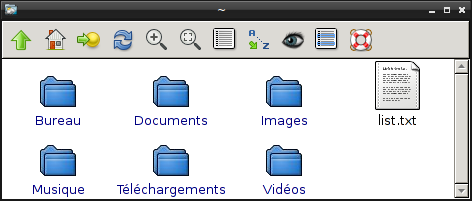
\includegraphics[width=0.7\textwidth]{rox1}
  \caption{\footnotesize{Le répertoire personnel /home/martin.albert}}
  \label{fig:rox1}
\end{figure}
Sous Unix (et donc sous GNU/Linux aussi), tous les fichiers sont regroupés dans une arborescence unique ; le sommet de cette arborescence est un répertoire appelé racine\footnote{Oui, en informatique les arbres poussent à l'envers, les racines sont en haut et les feuilles en bas.} et noté /.\par
Cette racine possède plusieurs sous-répertoires (voir figure \ref{fig:rox2}) dont les principaux sont :
\begin{description}
\item[home :] qui contient les données de tous les utilisateurs, il y a un sous-répertoire par utilisateur ;
\item[bin :] une partie des programmes installés ;
\item[mnt et media :] c'est ici qu'on retrouve les données stockées sur les autres disques durs, les clés USB, les lecteurs de médias \dots
\end{description}
\begin{figure}[ht]
  \centering
  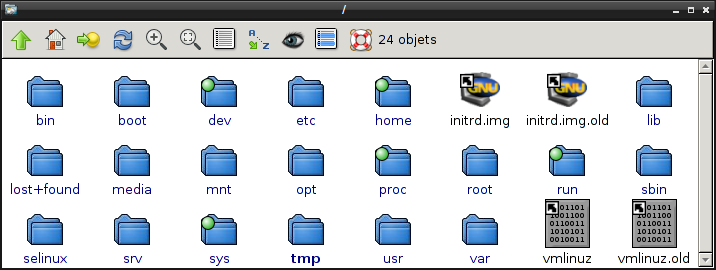
\includegraphics[width=0.7\textwidth]{rox2}
  \caption{\footnotesize{Le répertoire racine}}
  \label{fig:rox2}
\end{figure}
Sous Microsoft Windows, il y a une arborescence par périphérique de stockage de masse, chacun d'entre eux étant représenté par une lettre majuscule puis :\textbackslash. Par exemple C:\textbackslash pour le disque dur principal, D:\textbackslash pour le lecteur de DVD ou Blu Ray \dots. \par
Vous devez savoir vous repérer dans une arborescence notamment savoir retrouver votre répertoire personnel. Vous devez aussi savoir vous déplacer dans cette arborescence au moyen d'un shell graphique ou texte. Dans une shell Unix la commande pour changer de répertoire est \emph{cd} (pour change directory), pour remonter dans le répertoire parent il suffit d'utiliser \emph{cd ..}. le symbole \emph{..} représente le répertoire parent du répertoire courant qui lui est représenté par \emph{.} comme vous pouvez le voir sur la figure \ref{fig:shelltexte}.\par
De plus vous allez être rapidement amené à organiser votre propres données et un peu de méthode permettra de mieux vous repérer. N'hésitez pas à utiliser des sous répertoires pour classer les fichiers faisant partie d'une catégorie particulière. Par exemple dans votre répertoire travail, vous créez un sous-répertoire python ou vous pouvez stocker tous vos scripts python.\par
Un fichier n'est qu'une séquence finie d'octets, sans signification a priori : c'est le programme qui lira cette séquence d'octets qui décidera de la façon de l'utiliser. Sous Unix un répertoire est aussi un fichier qui ne contient qu'une liste de couples ($n$, $i$) où $n$ est le nom du fichier et $i$ son \emph{inode} qui permet d'avoir accès aux méta-données du fichier qui sont stockées dans la table des inodes :
\begin{itemize}
\item la date de création, de dernière modification et de dernière lecture ;
\item la taille du fichier ;
\item emplacement des données sur le disque.
\end{itemize}

. Ainsi on dit souvent que sous Unix tout est fichier (même les périphériques d'entrée sortie sont représentés par des fichiers).
\subsection{Droits d'accès}
En parcourant l'arborescence, Albert Martin remarque que dans le répertoire /home il y a trois autres répertoires : martin.albert qui est son répertoire personnel puis reine.benedicte et cancanier.jean qui sont les répertoires personnels de deux de ses camarades. Il décide de les visiter mais lorsqu'il clique sur le répertoire cancanier.jean il obtient le message d'erreur présenté sur la figure \ref{fig:erreur1}.
\begin{figure}[ht]
  \centering
  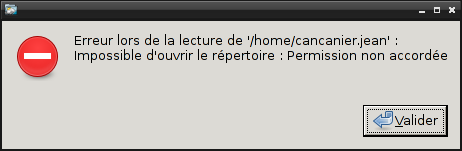
\includegraphics[width=0.6\textwidth]{erreur1}
  \caption{\footnotesize{Refus d'accès à /home/cancanier.jean}}
  \label{fig:erreur1}
\end{figure}
En revanche, il parvient à lire le répertoire /home/reine.benedicte. Celui-ci contient un fichier Lisez-moi.txt qu'Albert Martin parvient à ouvrir. Avec un éditeur de texte, il réussit à éditer le fichier mais lorsqu’il essaie de l’enregistrer, il obtient un message d’erreur présenté sur la figure \ref{fig:erreur2}. Le problème persiste s'il essaie d'enregistrer le fichier sous un autre nom.\par
\begin{wrapfigure}{r}{0.4\textwidth}
  \centering
  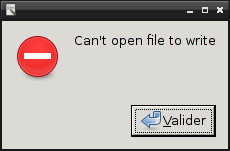
\includegraphics[width=0.325\textwidth]{erreur2}
  \caption{\footnotesize{Échec de l'enregistrement d'un fichier protégé en écriture}}
  \label{fig:erreur2}
\end{wrapfigure}
Chaque entrée de la table des inodes comporte, en plus des méta-données déjà mentionnées, les droits d'accès accordés aux utilisateurs du système. Ces droits ou permissions précisent qui à quels droits sur le fichier ou le répertoire concerné. Ces permissions sont accessibles avec la commande \emph{ls -l} dans un shell texte ou alors avec un clic droit sur le fichier ou répertoire concerné dans un shell graphique.\par
Ainsi, si on regarde les permissions de /home/cancanier.jean, les droits sont les suivants (voir figure \ref{fig:droit1}) :
\begin{figure}[ht]
  \centering
 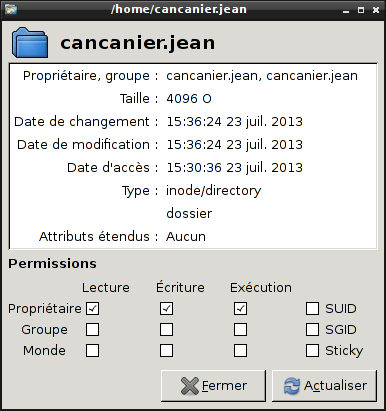
\includegraphics[width=0.6\textwidth]{droit1}
  \caption{\footnotesize{Les droits du répertoire /home/cancanier.jean}}
  \label{fig:droit1}  
\end{figure}
\begin{itemize}
\item le propriétaire du fichier est l'utilisateur cancanier.jean ;
\item le groupe auquel appartient le fichier est aussi cancanier.jean ;
\item le propriétaire du fichier peut accéder en lecture et en écriture au fichier ;
\item les autres utilisateurs n'ont aucun droit sur le fichier. 
\end{itemize}
Ainsi Albert Martin n'a pas les droits pour lire le contenu du répertoire /home/cancnier.jean d'où le premier message d'erreur (figure \ref{fig:erreur1}). \par
Dans le cas présenté figure \ref{fig:erreur2} Albert Martin essaie d'écrire sur un fichier sur lequel il n'a pas le droit d'écriture, comme on peut le constater figure \ref{fig:droit2}.
\begin{figure}[ht]
  \centering
  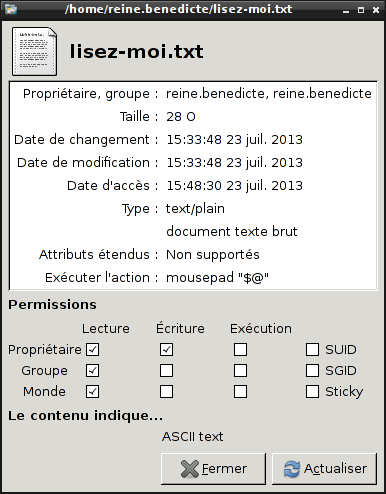
\includegraphics[width=0.6\textwidth]{droit2}
  \caption{\footnotesize{Les droits du fichier Lisez-moi.txt}}
  \label{fig:droit2}
\end{figure}
S'il essaye d'enregistrer le fichier sous un autre nom, il essayer d'écrire dans le répertoire /home/reine.benedicte sur lequel il n'a pas le droit en écriture, d'où le message d'erreur identique.\par
Tenter d'accéder aux données d'autrui peut être considéré comme une atteinte à la vie privée. De la même manière qu'on entre pas dans une maison inconnue même si la porte n'est pas verrouillée on ne cherche pas à accéder aux données d'une personne même s'il elle n'a pas bien définit les droits d'accès. Il convient d'en demander d'abord l'autorisation.\par
Passer outre une interdiction voire même se passer d'autorisation est pénalement répréhensible (art. 323-1 et suivants du code pénal). Et les peines encourues sont particulièrement lourdes : par exemple le simple fait d'accéder à un système informatique ou à des données en sachant qu'on n'en n'a pas l'autorisation, sans intention de commettre de dégâts, sans même commettre le moindre dégât involontaire, même si aucune protection n'est en place, est passible de 2 ans d'emprisonnement et 30 000 euros d'amende. 
%%% Local Variables: 
%%% mode: latex
%%% TeX-master: "cours-ipt"
%%% End: 












\end{document}













